\documentclass[twoside]{book}

% Packages required by doxygen
\usepackage{calc}
\usepackage{doxygen}
\usepackage{graphicx}
\usepackage[utf8]{inputenc}
\usepackage{makeidx}
\usepackage{multicol}
\usepackage{multirow}
\usepackage{textcomp}
\usepackage[table]{xcolor}

% Font selection
\usepackage[T1]{fontenc}
\usepackage{mathptmx}
\usepackage[scaled=.90]{helvet}
\usepackage{courier}
\usepackage{amssymb}
\usepackage{sectsty}
\renewcommand{\familydefault}{\sfdefault}
\allsectionsfont{%
  \fontseries{bc}\selectfont%
  \color{darkgray}%
}
\renewcommand{\DoxyLabelFont}{%
  \fontseries{bc}\selectfont%
  \color{darkgray}%
}

% Page & text layout
\usepackage{geometry}
\geometry{%
  a4paper,%
  top=2.5cm,%
  bottom=2.5cm,%
  left=2.5cm,%
  right=2.5cm%
}
\tolerance=750
\hfuzz=15pt
\hbadness=750
\setlength{\emergencystretch}{15pt}
\setlength{\parindent}{0cm}
\setlength{\parskip}{0.2cm}
\makeatletter
\renewcommand{\paragraph}{%
  \@startsection{paragraph}{4}{0ex}{-1.0ex}{1.0ex}{%
    \normalfont\normalsize\bfseries\SS@parafont%
  }%
}
\renewcommand{\subparagraph}{%
  \@startsection{subparagraph}{5}{0ex}{-1.0ex}{1.0ex}{%
    \normalfont\normalsize\bfseries\SS@subparafont%
  }%
}
\makeatother

% Headers & footers
\usepackage{fancyhdr}
\pagestyle{fancyplain}
\fancyhead[LE]{\fancyplain{}{\bfseries\thepage}}
\fancyhead[CE]{\fancyplain{}{}}
\fancyhead[RE]{\fancyplain{}{\bfseries\leftmark}}
\fancyhead[LO]{\fancyplain{}{\bfseries\rightmark}}
\fancyhead[CO]{\fancyplain{}{}}
\fancyhead[RO]{\fancyplain{}{\bfseries\thepage}}
\fancyfoot[LE]{\fancyplain{}{}}
\fancyfoot[CE]{\fancyplain{}{}}
\fancyfoot[RE]{\fancyplain{}{\bfseries\scriptsize Generated on Fri May 8 2015 18\-:41\-:32 for Breakout by Doxygen }}
\fancyfoot[LO]{\fancyplain{}{\bfseries\scriptsize Generated on Fri May 8 2015 18\-:41\-:32 for Breakout by Doxygen }}
\fancyfoot[CO]{\fancyplain{}{}}
\fancyfoot[RO]{\fancyplain{}{}}
\renewcommand{\footrulewidth}{0.4pt}
\renewcommand{\chaptermark}[1]{%
  \markboth{#1}{}%
}
\renewcommand{\sectionmark}[1]{%
  \markright{\thesection\ #1}%
}

% Indices & bibliography
\usepackage{natbib}
\usepackage[titles]{tocloft}
\setcounter{tocdepth}{3}
\setcounter{secnumdepth}{5}
\makeindex

% Hyperlinks (required, but should be loaded last)
\usepackage{ifpdf}
\ifpdf
  \usepackage[pdftex,pagebackref=true]{hyperref}
\else
  \usepackage[ps2pdf,pagebackref=true]{hyperref}
\fi
\hypersetup{%
  colorlinks=true,%
  linkcolor=blue,%
  citecolor=blue,%
  unicode%
}

% Custom commands
\newcommand{\clearemptydoublepage}{%
  \newpage{\pagestyle{empty}\cleardoublepage}%
}


%===== C O N T E N T S =====

\begin{document}

% Titlepage & ToC
\hypersetup{pageanchor=false}
\pagenumbering{roman}
\begin{titlepage}
\vspace*{7cm}
\begin{center}%
{\Large Breakout }\\
\vspace*{1cm}
{\large Generated by Doxygen 1.8.6}\\
\vspace*{0.5cm}
{\small Fri May 8 2015 18:41:32}\\
\end{center}
\end{titlepage}
\clearemptydoublepage
\tableofcontents
\clearemptydoublepage
\pagenumbering{arabic}
\hypersetup{pageanchor=true}

%--- Begin generated contents ---
\chapter{Breakout Documentation File}
\label{index}\hypertarget{index}{}\subsection*{Author}

Nicole Zhang

\subsection*{Documentation and Game Overview}

Here you will find documentation on the game Breakout, created for the individual project assignment for C\-S\-C\-I 3081\-W. The objective of the game is to break all the bricks in the game, displayed as a beautiful rainbow at the top half of the screen. A ball bounces back and forth around the environment and destroys any bricks it comes in contact with, and the player controls a paddle at the bottom of the screen to bounce the ball back up towards the bricks. Instructions on how to control the paddle and pause the game are displayed in the \char`\"{}\-Controls\char`\"{} window when the game is run. If the ball passes below the paddle and hits the bottom of the screen, the player loses a life. Popularized by the Activision's 2014 hit \char`\"{}\-Call of Duty\-: Advanced Warfare\char`\"{}, the option to press \char`\"{}\-F\char`\"{} to pay respects is available when the player loses a life. The player gets three total lives to complete the objective and break all the bricks. If the player loses all three lives before breaking all the bricks, it's game over. 


\chapter{R\-E\-A\-D\-M\-E}
\label{md_README}
\hypertarget{md_README}{}
T\-H\-I\-S I\-S B\-R\-E\-A\-K\-O\-U\-T 
\chapter{Hierarchical Index}
\section{Class Hierarchy}
This inheritance list is sorted roughly, but not completely, alphabetically\-:\begin{DoxyCompactList}
\item \contentsline{section}{Base\-Gfx\-App}{\pageref{classBaseGfxApp}}{}
\begin{DoxyCompactList}
\item \contentsline{section}{Simulation}{\pageref{classSimulation}}{}
\end{DoxyCompactList}
\item \contentsline{section}{Environment\-Class}{\pageref{classEnvironmentClass}}{}
\item \contentsline{section}{Physical\-Object\-Class}{\pageref{classPhysicalObjectClass}}{}
\item \contentsline{section}{Rendering\-Window\-Class}{\pageref{classRenderingWindowClass}}{}
\end{DoxyCompactList}

\chapter{Class Index}
\section{Class List}
Here are the classes, structs, unions and interfaces with brief descriptions\-:\begin{DoxyCompactList}
\item\contentsline{section}{\hyperlink{classBaseGfxApp}{Base\-Gfx\-App} }{\pageref{classBaseGfxApp}}{}
\item\contentsline{section}{\hyperlink{classEnvironmentClass}{Environment\-Class} }{\pageref{classEnvironmentClass}}{}
\item\contentsline{section}{\hyperlink{classPhysicalObjectClass}{Physical\-Object\-Class} }{\pageref{classPhysicalObjectClass}}{}
\item\contentsline{section}{\hyperlink{classRenderingWindowClass}{Rendering\-Window\-Class} }{\pageref{classRenderingWindowClass}}{}
\item\contentsline{section}{\hyperlink{classSimulation}{Simulation} }{\pageref{classSimulation}}{}
\end{DoxyCompactList}

\chapter{File Index}
\section{File List}
Here is a list of all documented files with brief descriptions\-:\begin{DoxyCompactList}
\item\contentsline{section}{\hyperlink{BaseGfxApp_8h}{Base\-Gfx\-App.\-h} \\*The basic application class for C\-Sci-\/3081 project. Uses G\-L\-U\-T and G\-L\-U\-I and wraps them in a nice C++ interface }{\pageref{BaseGfxApp_8h}}{}
\item\contentsline{section}{\hyperlink{EnvironmentClass_8cpp}{Environment\-Class.\-cpp} \\*Manages and controls object movement and behavior }{\pageref{EnvironmentClass_8cpp}}{}
\item\contentsline{section}{\hyperlink{EnvironmentClass_8h}{Environment\-Class.\-h} \\*The class that controls the environment that the objects move in }{\pageref{EnvironmentClass_8h}}{}
\item\contentsline{section}{\hyperlink{main_8cpp}{main.\-cpp} \\*Driver file for robot class }{\pageref{main_8cpp}}{}
\item\contentsline{section}{\hyperlink{PhysicalObjectClass_8cpp}{Physical\-Object\-Class.\-cpp} \\*The class that creates all physical objects }{\pageref{PhysicalObjectClass_8cpp}}{}
\item\contentsline{section}{\hyperlink{PhysicalObjectClass_8h}{Physical\-Object\-Class.\-h} \\*The class that creates all physical objects }{\pageref{PhysicalObjectClass_8h}}{}
\item\contentsline{section}{\hyperlink{RenderingWindowClass_8cpp}{Rendering\-Window\-Class.\-cpp} \\*Interface between the graphics and \hyperlink{classEnvironmentClass}{Environment\-Class} }{\pageref{RenderingWindowClass_8cpp}}{}
\item\contentsline{section}{\hyperlink{RenderingWindowClass_8h}{Rendering\-Window\-Class.\-h} \\*Interface between the graphics and \hyperlink{classEnvironmentClass}{Environment\-Class} }{\pageref{RenderingWindowClass_8h}}{}
\item\contentsline{section}{\hyperlink{Simulation_8cpp}{Simulation.\-cpp} \\*Contains \hyperlink{classSimulation}{Simulation} class definitions }{\pageref{Simulation_8cpp}}{}
\item\contentsline{section}{\hyperlink{Simulation_8h}{Simulation.\-h} \\*Main application class for the robot simulation }{\pageref{Simulation_8h}}{}
\end{DoxyCompactList}

\chapter{Class Documentation}
\hypertarget{classBaseGfxApp}{\section{Base\-Gfx\-App Class Reference}
\label{classBaseGfxApp}\index{Base\-Gfx\-App@{Base\-Gfx\-App}}
}


Inheritance diagram for Base\-Gfx\-App\-:\nopagebreak
\begin{figure}[H]
\begin{center}
\leavevmode
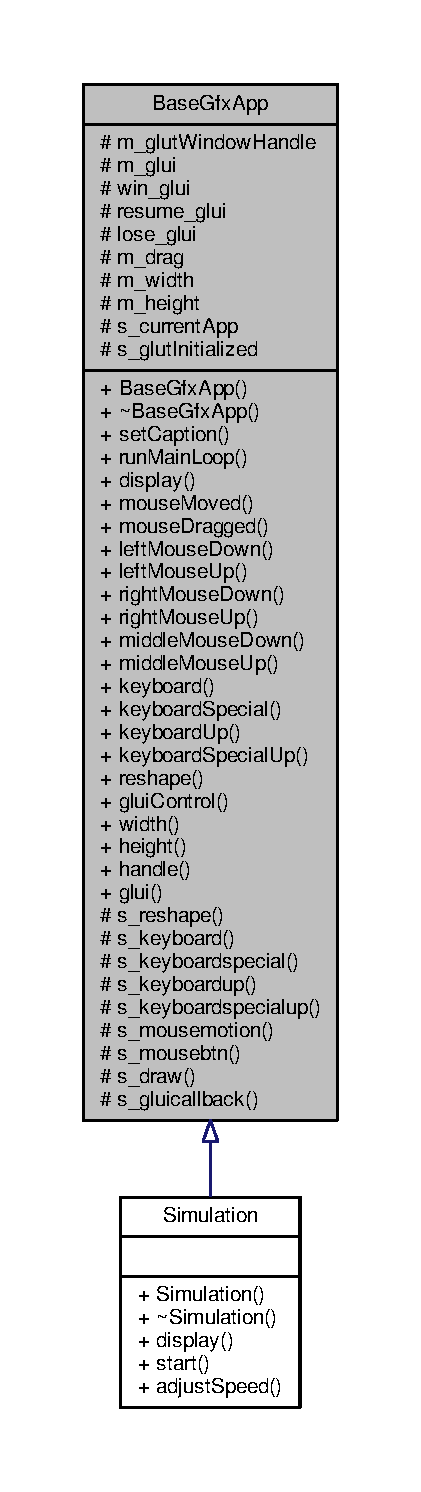
\includegraphics[height=550pt]{classBaseGfxApp__inherit__graph}
\end{center}
\end{figure}


Collaboration diagram for Base\-Gfx\-App\-:\nopagebreak
\begin{figure}[H]
\begin{center}
\leavevmode
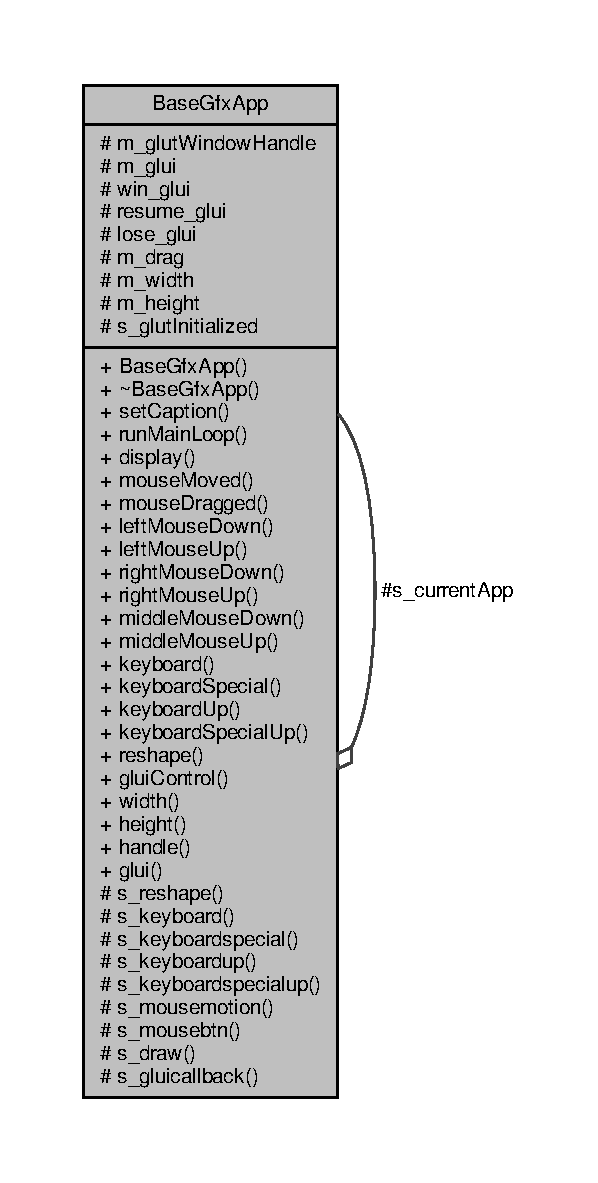
\includegraphics[height=550pt]{classBaseGfxApp__coll__graph}
\end{center}
\end{figure}
\subsection*{Public Member Functions}
\begin{DoxyCompactItemize}
\item 
\hypertarget{classBaseGfxApp_a534a4b5293a35947fdae3805a103541d}{{\bfseries Base\-Gfx\-App} (int argc, char $\ast$argv\mbox{[}$\,$\mbox{]}, int width, int height, int x, int y, int glut\-Flags, bool create\-G\-L\-U\-I\-Win, int glui\-Win\-X, int glui\-Win\-Y)}\label{classBaseGfxApp_a534a4b5293a35947fdae3805a103541d}

\item 
\hypertarget{classBaseGfxApp_a4b3b1a475b7f2babaf1b477c34b15fb1}{void {\bfseries set\-Caption} (const std\-::string \&caption)}\label{classBaseGfxApp_a4b3b1a475b7f2babaf1b477c34b15fb1}

\item 
\hypertarget{classBaseGfxApp_acda031916c00d56c2dc901e2653e3083}{void {\bfseries run\-Main\-Loop} ()}\label{classBaseGfxApp_acda031916c00d56c2dc901e2653e3083}

\item 
\hypertarget{classBaseGfxApp_ac8de2d5a955582547af5619b771b4d6d}{virtual void {\bfseries display} ()}\label{classBaseGfxApp_ac8de2d5a955582547af5619b771b4d6d}

\item 
\hypertarget{classBaseGfxApp_a0956b82d7fa58b623c498aea7073dbba}{virtual void {\bfseries mouse\-Moved} (int x, int y)}\label{classBaseGfxApp_a0956b82d7fa58b623c498aea7073dbba}

\item 
\hypertarget{classBaseGfxApp_abb23f716dd6612b3a72938e41525d338}{virtual void {\bfseries mouse\-Dragged} (int x, int y)}\label{classBaseGfxApp_abb23f716dd6612b3a72938e41525d338}

\item 
\hypertarget{classBaseGfxApp_aaaccf5a5e923a9465441a5ee712424a8}{virtual void {\bfseries left\-Mouse\-Down} (int x, int y)}\label{classBaseGfxApp_aaaccf5a5e923a9465441a5ee712424a8}

\item 
\hypertarget{classBaseGfxApp_a0a2961a932b02b2f9d7d0bb408f6fb51}{virtual void {\bfseries left\-Mouse\-Up} (int x, int y)}\label{classBaseGfxApp_a0a2961a932b02b2f9d7d0bb408f6fb51}

\item 
\hypertarget{classBaseGfxApp_afa87e6a71220945e41f0424e540125d9}{virtual void {\bfseries right\-Mouse\-Down} (int x, int y)}\label{classBaseGfxApp_afa87e6a71220945e41f0424e540125d9}

\item 
\hypertarget{classBaseGfxApp_a812643d563522a993457dd565c33f8f6}{virtual void {\bfseries right\-Mouse\-Up} (int x, int y)}\label{classBaseGfxApp_a812643d563522a993457dd565c33f8f6}

\item 
\hypertarget{classBaseGfxApp_a2c98cae9bb5ad1fb1832a6d4812670f8}{virtual void {\bfseries middle\-Mouse\-Down} (int x, int y)}\label{classBaseGfxApp_a2c98cae9bb5ad1fb1832a6d4812670f8}

\item 
\hypertarget{classBaseGfxApp_a00fc05e8d9629b72302b5adf014bdb0c}{virtual void {\bfseries middle\-Mouse\-Up} (int x, int y)}\label{classBaseGfxApp_a00fc05e8d9629b72302b5adf014bdb0c}

\item 
\hypertarget{classBaseGfxApp_a6d91e0cb7a3d48cad33956efe7eb36ca}{virtual void {\bfseries keyboard} (unsigned char c, int x, int y)}\label{classBaseGfxApp_a6d91e0cb7a3d48cad33956efe7eb36ca}

\item 
\hypertarget{classBaseGfxApp_a345566e62c9e4ec3705ec4d1c4c75f1f}{virtual void {\bfseries keyboard\-Special} (int key, int x, int y)}\label{classBaseGfxApp_a345566e62c9e4ec3705ec4d1c4c75f1f}

\item 
\hypertarget{classBaseGfxApp_acc4a40ce11edd6b6660a19cb4802a2bf}{virtual void {\bfseries keyboard\-Up} (unsigned char c, int x, int y)}\label{classBaseGfxApp_acc4a40ce11edd6b6660a19cb4802a2bf}

\item 
\hypertarget{classBaseGfxApp_afd14b435ff93b1e7f461cb8bd1a6fd59}{virtual void {\bfseries keyboard\-Special\-Up} (int key, int x, int y)}\label{classBaseGfxApp_afd14b435ff93b1e7f461cb8bd1a6fd59}

\item 
\hypertarget{classBaseGfxApp_a5d8d5d778a8aecd7f5f8e9c87f4c3d20}{virtual void {\bfseries reshape} (int width, int height)}\label{classBaseGfxApp_a5d8d5d778a8aecd7f5f8e9c87f4c3d20}

\item 
\hypertarget{classBaseGfxApp_a2978a7c358794c67df73b66776b2cef3}{virtual void {\bfseries glui\-Control} (int control\-I\-D)}\label{classBaseGfxApp_a2978a7c358794c67df73b66776b2cef3}

\item 
\hypertarget{classBaseGfxApp_ace089a1a94fb6bb0bc17e1b7fa48e05d}{int {\bfseries width} () const }\label{classBaseGfxApp_ace089a1a94fb6bb0bc17e1b7fa48e05d}

\item 
\hypertarget{classBaseGfxApp_aa253dbe16a20c40e0a1bf8ff942ceea3}{int {\bfseries height} () const }\label{classBaseGfxApp_aa253dbe16a20c40e0a1bf8ff942ceea3}

\item 
\hypertarget{classBaseGfxApp_ae9779f948eff6f45beec08091e98a803}{int {\bfseries handle} ()}\label{classBaseGfxApp_ae9779f948eff6f45beec08091e98a803}

\item 
\hypertarget{classBaseGfxApp_ac721a0fedce80308c5c0e5695016e95d}{G\-L\-U\-I $\ast$ {\bfseries glui} ()}\label{classBaseGfxApp_ac721a0fedce80308c5c0e5695016e95d}

\end{DoxyCompactItemize}
\subsection*{Static Protected Member Functions}
\begin{DoxyCompactItemize}
\item 
\hypertarget{classBaseGfxApp_a5fe6a77d37044cbe28647ed3391bbb7a}{static void {\bfseries s\-\_\-reshape} (int width, int height)}\label{classBaseGfxApp_a5fe6a77d37044cbe28647ed3391bbb7a}

\item 
static void \hyperlink{classBaseGfxApp_a52edb2569227319feb68779844e7d857}{s\-\_\-keyboard} (unsigned char c, int x, int y)
\begin{DoxyCompactList}\small\item\em Perform keyboard press actions. \end{DoxyCompactList}\item 
static void \hyperlink{classBaseGfxApp_a1e8d90a4faab60300ddf2a4ea9b83115}{s\-\_\-keyboardspecial} (int key, int x, int y)
\begin{DoxyCompactList}\small\item\em Perform special keyboard press actions. \end{DoxyCompactList}\item 
\hypertarget{classBaseGfxApp_aa1ca205af9d6cee33949f2e6adf4c923}{static void {\bfseries s\-\_\-keyboardup} (unsigned char c, int x, int y)}\label{classBaseGfxApp_aa1ca205af9d6cee33949f2e6adf4c923}

\item 
static void \hyperlink{classBaseGfxApp_a0e4dfe006f3cc9126c1cc8ad32784f75}{s\-\_\-keyboardspecialup} (int key, int x, int y)
\begin{DoxyCompactList}\small\item\em Determines which side of a brick has been hit. \end{DoxyCompactList}\item 
\hypertarget{classBaseGfxApp_a5e640f2394f7e038d0dd2b469d5c2e24}{static void {\bfseries s\-\_\-mousemotion} (int x, int y)}\label{classBaseGfxApp_a5e640f2394f7e038d0dd2b469d5c2e24}

\item 
\hypertarget{classBaseGfxApp_a22dd953bfb75add9fd0f8f2f8be535c5}{static void {\bfseries s\-\_\-mousebtn} (int b, int s, int x, int y)}\label{classBaseGfxApp_a22dd953bfb75add9fd0f8f2f8be535c5}

\item 
\hypertarget{classBaseGfxApp_a58415c6151a2a80e1fe2eaa9919a4dab}{static void {\bfseries s\-\_\-draw} ()}\label{classBaseGfxApp_a58415c6151a2a80e1fe2eaa9919a4dab}

\item 
\hypertarget{classBaseGfxApp_ad4a963321f1147d68369225ab0c7f32f}{static void {\bfseries s\-\_\-gluicallback} (int control\-I\-D)}\label{classBaseGfxApp_ad4a963321f1147d68369225ab0c7f32f}

\end{DoxyCompactItemize}
\subsection*{Protected Attributes}
\begin{DoxyCompactItemize}
\item 
int \hyperlink{classBaseGfxApp_ad8697d6fdd10e6f336c3a662016b4fa7}{m\-\_\-glut\-Window\-Handle}
\item 
\hypertarget{classBaseGfxApp_a6eb1673b80283727221da2242211af1d}{G\-L\-U\-I $\ast$ {\bfseries m\-\_\-glui}}\label{classBaseGfxApp_a6eb1673b80283727221da2242211af1d}

\item 
\hypertarget{classBaseGfxApp_a1df9b89d29761fd44208ba02decca76a}{G\-L\-U\-I $\ast$ {\bfseries win\-\_\-glui}}\label{classBaseGfxApp_a1df9b89d29761fd44208ba02decca76a}

\item 
\hypertarget{classBaseGfxApp_a6d8ae1f07cd0673627fef49baa27e4a8}{G\-L\-U\-I $\ast$ {\bfseries resume\-\_\-glui}}\label{classBaseGfxApp_a6d8ae1f07cd0673627fef49baa27e4a8}

\item 
\hypertarget{classBaseGfxApp_af1dd0795c8f5bdafe89050a42d9f96a4}{G\-L\-U\-I $\ast$ {\bfseries lose\-\_\-glui}}\label{classBaseGfxApp_af1dd0795c8f5bdafe89050a42d9f96a4}

\item 
\hypertarget{classBaseGfxApp_a2e70a389224f8affe7c137f7e20dc8c1}{bool {\bfseries m\-\_\-drag}}\label{classBaseGfxApp_a2e70a389224f8affe7c137f7e20dc8c1}

\item 
\hypertarget{classBaseGfxApp_a7e5ef1c8f25fe081b4a1fd4ce6a96e07}{int {\bfseries m\-\_\-width}}\label{classBaseGfxApp_a7e5ef1c8f25fe081b4a1fd4ce6a96e07}

\item 
\hypertarget{classBaseGfxApp_ac078e4fc20b5c2fe0c744966b850b412}{int {\bfseries m\-\_\-height}}\label{classBaseGfxApp_ac078e4fc20b5c2fe0c744966b850b412}

\end{DoxyCompactItemize}
\subsection*{Static Protected Attributes}
\begin{DoxyCompactItemize}
\item 
static \hyperlink{classBaseGfxApp}{Base\-Gfx\-App} $\ast$ \hyperlink{classBaseGfxApp_a65ba89b98af31e2649a0546631931000}{s\-\_\-current\-App} = N\-U\-L\-L
\item 
static bool \hyperlink{classBaseGfxApp_afa4690383ea27713016ef75b9fb1e42f}{s\-\_\-glut\-Initialized} = false
\end{DoxyCompactItemize}


\subsection{Member Function Documentation}
\hypertarget{classBaseGfxApp_a52edb2569227319feb68779844e7d857}{\index{Base\-Gfx\-App@{Base\-Gfx\-App}!s\-\_\-keyboard@{s\-\_\-keyboard}}
\index{s\-\_\-keyboard@{s\-\_\-keyboard}!BaseGfxApp@{Base\-Gfx\-App}}
\subsubsection[{s\-\_\-keyboard}]{\setlength{\rightskip}{0pt plus 5cm}void Base\-Gfx\-App\-::s\-\_\-keyboard (
\begin{DoxyParamCaption}
\item[{unsigned char}]{c, }
\item[{int}]{x, }
\item[{int}]{y}
\end{DoxyParamCaption}
)\hspace{0.3cm}{\ttfamily [static]}, {\ttfamily [protected]}}}\label{classBaseGfxApp_a52edb2569227319feb68779844e7d857}


Perform keyboard press actions. 

Pauses or resumes the simulation when spacebar is pressed, depending on the current flag status.


\begin{DoxyParams}{Parameters}
{\em c} & character pressed \\
\hline
{\em x} & mouse x location \\
\hline
{\em y} & mouse y location\\
\hline
\end{DoxyParams}
\begin{DoxyAuthor}{Author}
Nicole Zhang 
\end{DoxyAuthor}
\hypertarget{classBaseGfxApp_a1e8d90a4faab60300ddf2a4ea9b83115}{\index{Base\-Gfx\-App@{Base\-Gfx\-App}!s\-\_\-keyboardspecial@{s\-\_\-keyboardspecial}}
\index{s\-\_\-keyboardspecial@{s\-\_\-keyboardspecial}!BaseGfxApp@{Base\-Gfx\-App}}
\subsubsection[{s\-\_\-keyboardspecial}]{\setlength{\rightskip}{0pt plus 5cm}void Base\-Gfx\-App\-::s\-\_\-keyboardspecial (
\begin{DoxyParamCaption}
\item[{int}]{key, }
\item[{int}]{x, }
\item[{int}]{y}
\end{DoxyParamCaption}
)\hspace{0.3cm}{\ttfamily [static]}, {\ttfamily [protected]}}}\label{classBaseGfxApp_a1e8d90a4faab60300ddf2a4ea9b83115}


Perform special keyboard press actions. 

Moves the paddle left or right when the left or right arrow key is pressed.


\begin{DoxyParams}{Parameters}
{\em key} & key pressed \\
\hline
{\em x} & mouse x location \\
\hline
{\em y} & mouse y location\\
\hline
\end{DoxyParams}
\begin{DoxyAuthor}{Author}
Nicole Zhang 
\end{DoxyAuthor}
\hypertarget{classBaseGfxApp_a0e4dfe006f3cc9126c1cc8ad32784f75}{\index{Base\-Gfx\-App@{Base\-Gfx\-App}!s\-\_\-keyboardspecialup@{s\-\_\-keyboardspecialup}}
\index{s\-\_\-keyboardspecialup@{s\-\_\-keyboardspecialup}!BaseGfxApp@{Base\-Gfx\-App}}
\subsubsection[{s\-\_\-keyboardspecialup}]{\setlength{\rightskip}{0pt plus 5cm}void Base\-Gfx\-App\-::s\-\_\-keyboardspecialup (
\begin{DoxyParamCaption}
\item[{int}]{key, }
\item[{int}]{x, }
\item[{int}]{y}
\end{DoxyParamCaption}
)\hspace{0.3cm}{\ttfamily [static]}, {\ttfamily [protected]}}}\label{classBaseGfxApp_a0e4dfe006f3cc9126c1cc8ad32784f75}


Determines which side of a brick has been hit. 

The paddle stops moving when the left or right arrow key are released.


\begin{DoxyParams}{Parameters}
{\em key} & key released \\
\hline
{\em x} & mouse x location \\
\hline
{\em y} & mouse y location\\
\hline
\end{DoxyParams}
\begin{DoxyAuthor}{Author}
Nicole Zhang 
\end{DoxyAuthor}


\subsection{Member Data Documentation}
\hypertarget{classBaseGfxApp_ad8697d6fdd10e6f336c3a662016b4fa7}{\index{Base\-Gfx\-App@{Base\-Gfx\-App}!m\-\_\-glut\-Window\-Handle@{m\-\_\-glut\-Window\-Handle}}
\index{m\-\_\-glut\-Window\-Handle@{m\-\_\-glut\-Window\-Handle}!BaseGfxApp@{Base\-Gfx\-App}}
\subsubsection[{m\-\_\-glut\-Window\-Handle}]{\setlength{\rightskip}{0pt plus 5cm}int Base\-Gfx\-App\-::m\-\_\-glut\-Window\-Handle\hspace{0.3cm}{\ttfamily [protected]}}}\label{classBaseGfxApp_ad8697d6fdd10e6f336c3a662016b4fa7}
Underlying glut window handle \hypertarget{classBaseGfxApp_a65ba89b98af31e2649a0546631931000}{\index{Base\-Gfx\-App@{Base\-Gfx\-App}!s\-\_\-current\-App@{s\-\_\-current\-App}}
\index{s\-\_\-current\-App@{s\-\_\-current\-App}!BaseGfxApp@{Base\-Gfx\-App}}
\subsubsection[{s\-\_\-current\-App}]{\setlength{\rightskip}{0pt plus 5cm}{\bf Base\-Gfx\-App} $\ast$ Base\-Gfx\-App\-::s\-\_\-current\-App = N\-U\-L\-L\hspace{0.3cm}{\ttfamily [static]}, {\ttfamily [protected]}}}\label{classBaseGfxApp_a65ba89b98af31e2649a0546631931000}
G\-L\-U\-T and G\-L\-U\-I event callbacks are sent to the current window/app. Right now, there is only one window anyway (not counting the G\-L\-U\-I U\-I window.. in the future could be extended to support more windows. In any case, some structure like this is always needed when using glut with C++, since the glut callbacks must be either global or static functions. \hypertarget{classBaseGfxApp_afa4690383ea27713016ef75b9fb1e42f}{\index{Base\-Gfx\-App@{Base\-Gfx\-App}!s\-\_\-glut\-Initialized@{s\-\_\-glut\-Initialized}}
\index{s\-\_\-glut\-Initialized@{s\-\_\-glut\-Initialized}!BaseGfxApp@{Base\-Gfx\-App}}
\subsubsection[{s\-\_\-glut\-Initialized}]{\setlength{\rightskip}{0pt plus 5cm}bool Base\-Gfx\-App\-::s\-\_\-glut\-Initialized = false\hspace{0.3cm}{\ttfamily [static]}, {\ttfamily [protected]}}}\label{classBaseGfxApp_afa4690383ea27713016ef75b9fb1e42f}
Has glut\-Init been called? (only allowed once per program) 

The documentation for this class was generated from the following files\-:\begin{DoxyCompactItemize}
\item 
\hyperlink{BaseGfxApp_8h}{Base\-Gfx\-App.\-h}\item 
Base\-Gfx\-App.\-cpp\end{DoxyCompactItemize}

\hypertarget{classEnvironmentClass}{\section{Environment\-Class Class Reference}
\label{classEnvironmentClass}\index{Environment\-Class@{Environment\-Class}}
}


Collaboration diagram for Environment\-Class\-:\nopagebreak
\begin{figure}[H]
\begin{center}
\leavevmode
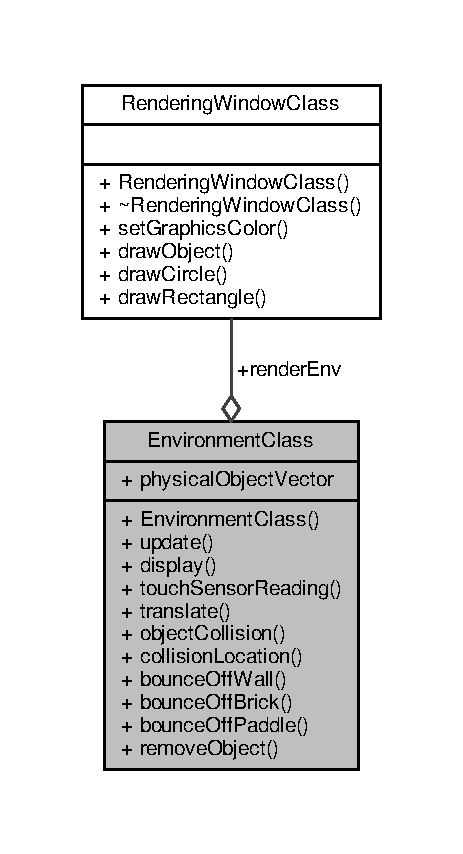
\includegraphics[width=222pt]{classEnvironmentClass__coll__graph}
\end{center}
\end{figure}
\subsection*{Public Member Functions}
\begin{DoxyCompactItemize}
\item 
\hypertarget{classEnvironmentClass_aa69ad01551a79f7326f005709061ff31}{\hyperlink{classEnvironmentClass_aa69ad01551a79f7326f005709061ff31}{Environment\-Class} ()}\label{classEnvironmentClass_aa69ad01551a79f7326f005709061ff31}

\begin{DoxyCompactList}\small\item\em Default constructor for \hyperlink{classEnvironmentClass}{Environment\-Class}. \end{DoxyCompactList}\item 
void \hyperlink{classEnvironmentClass_a7d992b6ef4e8b95542af1ae775be988a}{update} (double elapsed\-Time)
\begin{DoxyCompactList}\small\item\em Updates the environment and all its objects. \end{DoxyCompactList}\item 
void \hyperlink{classEnvironmentClass_a0c43d38e65c879efdad9f09a58835c77}{display} (double elapsed\-Time)
\begin{DoxyCompactList}\small\item\em Draw and displays objects and environment. \end{DoxyCompactList}\item 
int \hyperlink{classEnvironmentClass_a3acbe9866577efe3b66527babab09720}{touch\-Sensor\-Reading} (\hyperlink{classPhysicalObjectClass}{Physical\-Object\-Class} $\ast$ball)
\begin{DoxyCompactList}\small\item\em Collision detection. \end{DoxyCompactList}\item 
void \hyperlink{classEnvironmentClass_a0fa52a8dd735412f9d46f4e2499e8108}{translate} (\hyperlink{classPhysicalObjectClass}{Physical\-Object\-Class} $\ast$object, double elapsed\-Time)
\begin{DoxyCompactList}\small\item\em Moves the input object. \end{DoxyCompactList}\item 
void \hyperlink{classEnvironmentClass_a6ce1e78294fb94ac1fc27cf3ef1f0419}{object\-Collision} (\hyperlink{classPhysicalObjectClass}{Physical\-Object\-Class} $\ast$current\-Object, \hyperlink{classPhysicalObjectClass}{Physical\-Object\-Class} $\ast$hit\-Object, double elapsed\-Time)
\begin{DoxyCompactList}\small\item\em Performs wall collision movement. \end{DoxyCompactList}\item 
\hyperlink{EnvironmentClass_8h_aa884075f403706dceea29a61771a0d44}{Collision\-Type} \hyperlink{classEnvironmentClass_a75226d04d26221aa24cef7a00bce6ce2}{collision\-Location} (\hyperlink{classPhysicalObjectClass}{Physical\-Object\-Class} $\ast$ball, \hyperlink{classPhysicalObjectClass}{Physical\-Object\-Class} $\ast$brick)
\begin{DoxyCompactList}\small\item\em Determines which side of a brick has been hit. \end{DoxyCompactList}\item 
void \hyperlink{classEnvironmentClass_a1ed98b3b6278f232cf12f660b8adbc42}{bounce\-Off\-Wall} (\hyperlink{classPhysicalObjectClass}{Physical\-Object\-Class} $\ast$ball)
\begin{DoxyCompactList}\small\item\em Performs wall collision movement. \end{DoxyCompactList}\item 
void \hyperlink{classEnvironmentClass_a897de11455490caa445294c40db3347d}{bounce\-Off\-Brick} (\hyperlink{classPhysicalObjectClass}{Physical\-Object\-Class} $\ast$ball, \hyperlink{classPhysicalObjectClass}{Physical\-Object\-Class} $\ast$brick)
\begin{DoxyCompactList}\small\item\em Performs brick collision movement. \end{DoxyCompactList}\item 
void \hyperlink{classEnvironmentClass_a36b4ce6ee76f327dc2b5155228ccf177}{bounce\-Off\-Paddle} (\hyperlink{classPhysicalObjectClass}{Physical\-Object\-Class} $\ast$ball, \hyperlink{classPhysicalObjectClass}{Physical\-Object\-Class} $\ast$paddle)
\begin{DoxyCompactList}\small\item\em Performs paddle collision movement. \end{DoxyCompactList}\item 
void \hyperlink{classEnvironmentClass_a564160db6ba48653b24b3a42ce9d2d58}{remove\-Object} (\hyperlink{classPhysicalObjectClass}{Physical\-Object\-Class} $\ast$object)
\begin{DoxyCompactList}\small\item\em Removes the object from the simulation. \end{DoxyCompactList}\end{DoxyCompactItemize}
\subsection*{Public Attributes}
\begin{DoxyCompactItemize}
\item 
\hypertarget{classEnvironmentClass_a3735bf3dc818a03984620368f196b1d0}{std\-::vector\\*
$<$ \hyperlink{classPhysicalObjectClass}{Physical\-Object\-Class} $\ast$ $>$ {\bfseries physical\-Object\-Vector}}\label{classEnvironmentClass_a3735bf3dc818a03984620368f196b1d0}

\item 
\hypertarget{classEnvironmentClass_a403bb85973a4db56e0163686147dae8b}{\hyperlink{classRenderingWindowClass}{Rendering\-Window\-Class} $\ast$ {\bfseries render\-Env}}\label{classEnvironmentClass_a403bb85973a4db56e0163686147dae8b}

\end{DoxyCompactItemize}


\subsection{Member Function Documentation}
\hypertarget{classEnvironmentClass_a897de11455490caa445294c40db3347d}{\index{Environment\-Class@{Environment\-Class}!bounce\-Off\-Brick@{bounce\-Off\-Brick}}
\index{bounce\-Off\-Brick@{bounce\-Off\-Brick}!EnvironmentClass@{Environment\-Class}}
\subsubsection[{bounce\-Off\-Brick}]{\setlength{\rightskip}{0pt plus 5cm}void Environment\-Class\-::bounce\-Off\-Brick (
\begin{DoxyParamCaption}
\item[{{\bf Physical\-Object\-Class} $\ast$}]{ball, }
\item[{{\bf Physical\-Object\-Class} $\ast$}]{brick}
\end{DoxyParamCaption}
)}}\label{classEnvironmentClass_a897de11455490caa445294c40db3347d}


Performs brick collision movement. 

This function first determines which side of a brick the ball has collided with through the collision\-Location function. It then determines the new orientation the ball must have in order to have a natural looking bounce, which is based on its old orientation.


\begin{DoxyParams}{Parameters}
{\em ball} & the ball \\
\hline
{\em brick} & the brick being hit\\
\hline
\end{DoxyParams}
\begin{DoxyAuthor}{Author}
Nicole Zhang 
\end{DoxyAuthor}
\hypertarget{classEnvironmentClass_a36b4ce6ee76f327dc2b5155228ccf177}{\index{Environment\-Class@{Environment\-Class}!bounce\-Off\-Paddle@{bounce\-Off\-Paddle}}
\index{bounce\-Off\-Paddle@{bounce\-Off\-Paddle}!EnvironmentClass@{Environment\-Class}}
\subsubsection[{bounce\-Off\-Paddle}]{\setlength{\rightskip}{0pt plus 5cm}void Environment\-Class\-::bounce\-Off\-Paddle (
\begin{DoxyParamCaption}
\item[{{\bf Physical\-Object\-Class} $\ast$}]{ball, }
\item[{{\bf Physical\-Object\-Class} $\ast$}]{paddle}
\end{DoxyParamCaption}
)}}\label{classEnvironmentClass_a36b4ce6ee76f327dc2b5155228ccf177}


Performs paddle collision movement. 

This function finds where on the paddle the ball has collided with and determines its new orientation based on this information. The further away from the paddle's centerpoint the ball has collided with, the sharper the angle the ball will bounce back towards.


\begin{DoxyParams}{Parameters}
{\em ball} & the ball \\
\hline
{\em paddle} & the paddle\\
\hline
\end{DoxyParams}
\begin{DoxyAuthor}{Author}
Nicole Zhang 
\end{DoxyAuthor}
\hypertarget{classEnvironmentClass_a1ed98b3b6278f232cf12f660b8adbc42}{\index{Environment\-Class@{Environment\-Class}!bounce\-Off\-Wall@{bounce\-Off\-Wall}}
\index{bounce\-Off\-Wall@{bounce\-Off\-Wall}!EnvironmentClass@{Environment\-Class}}
\subsubsection[{bounce\-Off\-Wall}]{\setlength{\rightskip}{0pt plus 5cm}void Environment\-Class\-::bounce\-Off\-Wall (
\begin{DoxyParamCaption}
\item[{{\bf Physical\-Object\-Class} $\ast$}]{ball}
\end{DoxyParamCaption}
)}}\label{classEnvironmentClass_a1ed98b3b6278f232cf12f660b8adbc42}


Performs wall collision movement. 

This function performs collision movement when the ball has hit a wall. It first detects which wall it has hit and then bounces off in a natural manner, based on its old orientation. The ball is also translated inwards a bit in order to prevent clipping. If the ball has collided with the bottom wall, the ball does not bounce off but instead returns to the starting location and orientation. The paddle also returns to its starting location. In this case, a turn is lost and the game is paused, until the player presses \char`\"{}\-Start\char`\"{} again.


\begin{DoxyParams}{Parameters}
{\em ball} & the ball\\
\hline
\end{DoxyParams}
\begin{DoxyAuthor}{Author}
Nicole Zhang 
\end{DoxyAuthor}
\hypertarget{classEnvironmentClass_a75226d04d26221aa24cef7a00bce6ce2}{\index{Environment\-Class@{Environment\-Class}!collision\-Location@{collision\-Location}}
\index{collision\-Location@{collision\-Location}!EnvironmentClass@{Environment\-Class}}
\subsubsection[{collision\-Location}]{\setlength{\rightskip}{0pt plus 5cm}{\bf Collision\-Type} Environment\-Class\-::collision\-Location (
\begin{DoxyParamCaption}
\item[{{\bf Physical\-Object\-Class} $\ast$}]{ball, }
\item[{{\bf Physical\-Object\-Class} $\ast$}]{brick}
\end{DoxyParamCaption}
)}}\label{classEnvironmentClass_a75226d04d26221aa24cef7a00bce6ce2}


Determines which side of a brick has been hit. 

This function determines which side of a brick the ball is colliding with and returns the Collision\-Type enum indicating whether the left, right, top, or bottom side has been collided into. If no collision is detected, no\-Collision will be returned.


\begin{DoxyParams}{Parameters}
{\em ball} & the ball \\
\hline
{\em brick} & the brick being hit\\
\hline
\end{DoxyParams}
\begin{DoxyReturn}{Returns}
enum Collision\-Type location of collision
\end{DoxyReturn}
\begin{DoxyAuthor}{Author}
Nicole Zhang 
\end{DoxyAuthor}
\hypertarget{classEnvironmentClass_a0c43d38e65c879efdad9f09a58835c77}{\index{Environment\-Class@{Environment\-Class}!display@{display}}
\index{display@{display}!EnvironmentClass@{Environment\-Class}}
\subsubsection[{display}]{\setlength{\rightskip}{0pt plus 5cm}void Environment\-Class\-::display (
\begin{DoxyParamCaption}
\item[{double}]{elapsed\-Time}
\end{DoxyParamCaption}
)}}\label{classEnvironmentClass_a0c43d38e65c879efdad9f09a58835c77}


Draw and displays objects and environment. 

This function is constantly called from simulation. It displays and draws all the objects and calls the update function and effectively sets up the environment. It uses the elapsed time input to determine the amount of movement for each object. This function also draws the life indicator balls in the upper left corner of the simulation.


\begin{DoxyParams}{Parameters}
{\em elapsed\-Time} & amount of time passed since last update\\
\hline
\end{DoxyParams}
\begin{DoxyAuthor}{Author}
Nicole Zhang 
\end{DoxyAuthor}
\hypertarget{classEnvironmentClass_a6ce1e78294fb94ac1fc27cf3ef1f0419}{\index{Environment\-Class@{Environment\-Class}!object\-Collision@{object\-Collision}}
\index{object\-Collision@{object\-Collision}!EnvironmentClass@{Environment\-Class}}
\subsubsection[{object\-Collision}]{\setlength{\rightskip}{0pt plus 5cm}void Environment\-Class\-::object\-Collision (
\begin{DoxyParamCaption}
\item[{{\bf Physical\-Object\-Class} $\ast$}]{current\-Object, }
\item[{{\bf Physical\-Object\-Class} $\ast$}]{hit\-Object, }
\item[{double}]{elapsed\-Time}
\end{DoxyParamCaption}
)}}\label{classEnvironmentClass_a6ce1e78294fb94ac1fc27cf3ef1f0419}


Performs wall collision movement. 

This function determines whether the object being hit is a brick or a paddle. If it is a brick, it will remove the brick after performing the appropriate collision movement. If it is a paddle, then it will perform the paddle collision movement but the paddle not be removed from the simulation.


\begin{DoxyParams}{Parameters}
{\em current\-Object} & ball object \\
\hline
{\em hit\-Object} & object being hit \\
\hline
{\em elapsed\-Time} & elapsed time\\
\hline
\end{DoxyParams}
\begin{DoxyAuthor}{Author}
Nicole Zhang 
\end{DoxyAuthor}
\hypertarget{classEnvironmentClass_a564160db6ba48653b24b3a42ce9d2d58}{\index{Environment\-Class@{Environment\-Class}!remove\-Object@{remove\-Object}}
\index{remove\-Object@{remove\-Object}!EnvironmentClass@{Environment\-Class}}
\subsubsection[{remove\-Object}]{\setlength{\rightskip}{0pt plus 5cm}void Environment\-Class\-::remove\-Object (
\begin{DoxyParamCaption}
\item[{{\bf Physical\-Object\-Class} $\ast$}]{object}
\end{DoxyParamCaption}
)}}\label{classEnvironmentClass_a564160db6ba48653b24b3a42ce9d2d58}


Removes the object from the simulation. 

This function removes the input object from the simulation by erasing it from the Physical\-Object\-Vector.


\begin{DoxyParams}{Parameters}
{\em object} & the object that needs removing\\
\hline
\end{DoxyParams}
\begin{DoxyAuthor}{Author}
Nicholas Inman 
\end{DoxyAuthor}
\hypertarget{classEnvironmentClass_a3acbe9866577efe3b66527babab09720}{\index{Environment\-Class@{Environment\-Class}!touch\-Sensor\-Reading@{touch\-Sensor\-Reading}}
\index{touch\-Sensor\-Reading@{touch\-Sensor\-Reading}!EnvironmentClass@{Environment\-Class}}
\subsubsection[{touch\-Sensor\-Reading}]{\setlength{\rightskip}{0pt plus 5cm}int Environment\-Class\-::touch\-Sensor\-Reading (
\begin{DoxyParamCaption}
\item[{{\bf Physical\-Object\-Class} $\ast$}]{ball}
\end{DoxyParamCaption}
)}}\label{classEnvironmentClass_a3acbe9866577efe3b66527babab09720}


Collision detection. 

This function takes in the ball and checks if it's colliding with another object or a wall. It returns -\/1 if the ball is not colliding with anything, -\/2 if it is colliding with a wall, or the index of the object it is colliding with.


\begin{DoxyParams}{Parameters}
{\em ball} & the ball\\
\hline
\end{DoxyParams}
\begin{DoxyReturn}{Returns}
-\/1 if the ball is not colliding with anything -\/2 if the ball is colliding with a wall index of the object the ball is colliding with
\end{DoxyReturn}
\begin{DoxyAuthor}{Author}
Nicole Zhang 
\end{DoxyAuthor}
\hypertarget{classEnvironmentClass_a0fa52a8dd735412f9d46f4e2499e8108}{\index{Environment\-Class@{Environment\-Class}!translate@{translate}}
\index{translate@{translate}!EnvironmentClass@{Environment\-Class}}
\subsubsection[{translate}]{\setlength{\rightskip}{0pt plus 5cm}void Environment\-Class\-::translate (
\begin{DoxyParamCaption}
\item[{{\bf Physical\-Object\-Class} $\ast$}]{object, }
\item[{double}]{elapsed\-Time}
\end{DoxyParamCaption}
)}}\label{classEnvironmentClass_a0fa52a8dd735412f9d46f4e2499e8108}


Moves the input object. 

This function resets the location of the input object based on its speed, original location, orientation, and elapsed time.


\begin{DoxyParams}{Parameters}
{\em object} & the object being translated \\
\hline
{\em elapsed\-Time} & the amount of time passed\\
\hline
\end{DoxyParams}
\begin{DoxyAuthor}{Author}
Nicholas Inman 

Rachel Soble 

Nicole Zhang 
\end{DoxyAuthor}
\hypertarget{classEnvironmentClass_a7d992b6ef4e8b95542af1ae775be988a}{\index{Environment\-Class@{Environment\-Class}!update@{update}}
\index{update@{update}!EnvironmentClass@{Environment\-Class}}
\subsubsection[{update}]{\setlength{\rightskip}{0pt plus 5cm}void Environment\-Class\-::update (
\begin{DoxyParamCaption}
\item[{double}]{elapsed\-Time}
\end{DoxyParamCaption}
)}}\label{classEnvironmentClass_a7d992b6ef4e8b95542af1ae775be988a}


Updates the environment and all its objects. 

This function takes in one argument, elapsed\-Time, and iterates through the physical\-Objects array, calling move each time. Move then returns a double\mbox{[}2\mbox{]} array containing the direction and magnitude of movement. Based on which coordinate the object currently is in, it sets the object's new position.


\begin{DoxyParams}{Parameters}
{\em elapsed\-Time} & the amount of time passed\\
\hline
\end{DoxyParams}
\begin{DoxyAuthor}{Author}
Nicholas Inman 

Rachel Soble 

Nicole Zhang 
\end{DoxyAuthor}


The documentation for this class was generated from the following files\-:\begin{DoxyCompactItemize}
\item 
\hyperlink{EnvironmentClass_8h}{Environment\-Class.\-h}\item 
\hyperlink{EnvironmentClass_8cpp}{Environment\-Class.\-cpp}\end{DoxyCompactItemize}

\hypertarget{classPhysicalObjectClass}{\section{Physical\-Object\-Class Class Reference}
\label{classPhysicalObjectClass}\index{Physical\-Object\-Class@{Physical\-Object\-Class}}
}


Collaboration diagram for Physical\-Object\-Class\-:\nopagebreak
\begin{figure}[H]
\begin{center}
\leavevmode
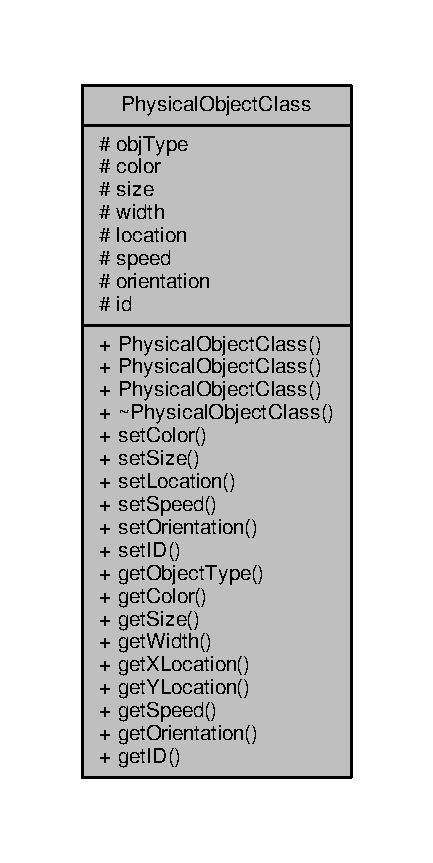
\includegraphics[width=208pt]{classPhysicalObjectClass__coll__graph}
\end{center}
\end{figure}
\subsection*{Public Member Functions}
\begin{DoxyCompactItemize}
\item 
\hypertarget{classPhysicalObjectClass_a960979388739197bbf20ac18d08d7021}{\hyperlink{classPhysicalObjectClass_a960979388739197bbf20ac18d08d7021}{Physical\-Object\-Class} ()}\label{classPhysicalObjectClass_a960979388739197bbf20ac18d08d7021}

\begin{DoxyCompactList}\small\item\em Default constructor for \hyperlink{classPhysicalObjectClass}{Physical\-Object\-Class}. \end{DoxyCompactList}\item 
\hyperlink{classPhysicalObjectClass_a563152ccd0d7b8f1de8d4db32c2576da}{Physical\-Object\-Class} (\hyperlink{PhysicalObjectClass_8h_a842c5e2e69277690b064bf363c017980}{Object\-Type} obj\-Type\-In, double x, double y, char color\-In)
\begin{DoxyCompactList}\small\item\em Primary constructor for \hyperlink{classPhysicalObjectClass}{Physical\-Object\-Class}. \end{DoxyCompactList}\item 
\hyperlink{classPhysicalObjectClass_a0e940ca39a50d9534a32c55dd89085d1}{Physical\-Object\-Class} (double x, double y)
\begin{DoxyCompactList}\small\item\em Constructor for life indicator balls. \end{DoxyCompactList}\item 
\hypertarget{classPhysicalObjectClass_a97db381b4e2e357eeb8aeeb580d0b7bd}{\hyperlink{classPhysicalObjectClass_a97db381b4e2e357eeb8aeeb580d0b7bd}{$\sim$\-Physical\-Object\-Class} ()}\label{classPhysicalObjectClass_a97db381b4e2e357eeb8aeeb580d0b7bd}

\begin{DoxyCompactList}\small\item\em Default destructor for \hyperlink{classPhysicalObjectClass}{Physical\-Object\-Class}. \end{DoxyCompactList}\item 
void \hyperlink{classPhysicalObjectClass_aed8b6e0511dd981e8161eabfc6705be1}{set\-Color} (char color\-In)
\begin{DoxyCompactList}\small\item\em Set the Physical\-Object color. \end{DoxyCompactList}\item 
void \hyperlink{classPhysicalObjectClass_a46784b1ccea116af39de1bdccf64328a}{set\-Size} (double size\-In)
\begin{DoxyCompactList}\small\item\em Set the Physical\-Object size. \end{DoxyCompactList}\item 
virtual void \hyperlink{classPhysicalObjectClass_a3f9833aa04aa438de63b82fc761910ba}{set\-Location} (double x, double y)
\begin{DoxyCompactList}\small\item\em Set the Physical\-Object location. \end{DoxyCompactList}\item 
void \hyperlink{classPhysicalObjectClass_ab8315565f193dd26f7069480d820a7c9}{set\-Speed} (double pps)
\begin{DoxyCompactList}\small\item\em Sets the Physical\-Object speed. \end{DoxyCompactList}\item 
void \hyperlink{classPhysicalObjectClass_a27ee3beb6442bcccced77ce20bee7b4c}{set\-Orientation} (double degrees)
\begin{DoxyCompactList}\small\item\em Sets the object orientation. \end{DoxyCompactList}\item 
void \hyperlink{classPhysicalObjectClass_a24a8cd79d7edfdd4e77518f8710560f5}{set\-I\-D} (int id\-In)
\begin{DoxyCompactList}\small\item\em Sets the object's I\-D in the env Physical\-Object vector. \end{DoxyCompactList}\item 
\hyperlink{PhysicalObjectClass_8h_a842c5e2e69277690b064bf363c017980}{Object\-Type} \hyperlink{classPhysicalObjectClass_a22607bc441c1f2eb12ac515dfcae7727}{get\-Object\-Type} ()
\begin{DoxyCompactList}\small\item\em Returns the object Object\-Type. \end{DoxyCompactList}\item 
char \hyperlink{classPhysicalObjectClass_aa77678e94120c33115c1ca0ab7c3b303}{get\-Color} ()
\begin{DoxyCompactList}\small\item\em Returns the object color. \end{DoxyCompactList}\item 
double \hyperlink{classPhysicalObjectClass_a32ef3ee72e567f832441d0d597fd2385}{get\-Size} ()
\begin{DoxyCompactList}\small\item\em Returns the object size. \end{DoxyCompactList}\item 
double \hyperlink{classPhysicalObjectClass_a12ade657d9d1cbf10249cde977519b39}{get\-Width} ()
\begin{DoxyCompactList}\small\item\em Returns the object width. \end{DoxyCompactList}\item 
double \hyperlink{classPhysicalObjectClass_a17eb882028d4b3a95d0fee9f13ce2f5f}{get\-X\-Location} ()
\begin{DoxyCompactList}\small\item\em Returns the object's x-\/position. \end{DoxyCompactList}\item 
double \hyperlink{classPhysicalObjectClass_a43b08ed49c8ea7c51660b85b1a8e64d6}{get\-Y\-Location} ()
\begin{DoxyCompactList}\small\item\em Returns the object's y-\/position. \end{DoxyCompactList}\item 
double \hyperlink{classPhysicalObjectClass_a778e1ed4b802bfb06382d0b15c09fd29}{get\-Speed} ()
\begin{DoxyCompactList}\small\item\em Returns the object's speed. \end{DoxyCompactList}\item 
double \hyperlink{classPhysicalObjectClass_a99126574824b46b85bc2f4b831864693}{get\-Orientation} ()
\begin{DoxyCompactList}\small\item\em Returns object orientation. \end{DoxyCompactList}\item 
int \hyperlink{classPhysicalObjectClass_a73e1b1feb39c9d9252b0e2ef282a9e33}{get\-I\-D} ()
\begin{DoxyCompactList}\small\item\em Returns the object's I\-D in the env Physical\-Object vector. \end{DoxyCompactList}\end{DoxyCompactItemize}
\subsection*{Protected Attributes}
\begin{DoxyCompactItemize}
\item 
\hypertarget{classPhysicalObjectClass_ac8957c2b2d552988d9dc54c69147ffe8}{\hyperlink{PhysicalObjectClass_8h_a842c5e2e69277690b064bf363c017980}{Object\-Type} {\bfseries obj\-Type}}\label{classPhysicalObjectClass_ac8957c2b2d552988d9dc54c69147ffe8}

\item 
\hypertarget{classPhysicalObjectClass_a876fd288ad5f2de8672a0b5b5f3a335d}{char {\bfseries color}}\label{classPhysicalObjectClass_a876fd288ad5f2de8672a0b5b5f3a335d}

\item 
\hypertarget{classPhysicalObjectClass_a6cdaa6e2955344d25705a0fe7b43ca20}{double {\bfseries size}}\label{classPhysicalObjectClass_a6cdaa6e2955344d25705a0fe7b43ca20}

\item 
\hypertarget{classPhysicalObjectClass_a6c432a38089211869dcd30b2e702ce30}{double {\bfseries width}}\label{classPhysicalObjectClass_a6c432a38089211869dcd30b2e702ce30}

\item 
\hypertarget{classPhysicalObjectClass_afd7ab3d3930ed86d0cefeede8332a396}{double {\bfseries location} \mbox{[}2\mbox{]}}\label{classPhysicalObjectClass_afd7ab3d3930ed86d0cefeede8332a396}

\item 
\hypertarget{classPhysicalObjectClass_aceb602dbf5f6539d843ee2deb09b276c}{double {\bfseries speed}}\label{classPhysicalObjectClass_aceb602dbf5f6539d843ee2deb09b276c}

\item 
\hypertarget{classPhysicalObjectClass_a769340a4297c6bda4b0191cccfd4e8fe}{double {\bfseries orientation}}\label{classPhysicalObjectClass_a769340a4297c6bda4b0191cccfd4e8fe}

\item 
\hypertarget{classPhysicalObjectClass_a7ef14013e26bcc16fcce2b24eb9c203b}{int {\bfseries id}}\label{classPhysicalObjectClass_a7ef14013e26bcc16fcce2b24eb9c203b}

\end{DoxyCompactItemize}


\subsection{Constructor \& Destructor Documentation}
\hypertarget{classPhysicalObjectClass_a563152ccd0d7b8f1de8d4db32c2576da}{\index{Physical\-Object\-Class@{Physical\-Object\-Class}!Physical\-Object\-Class@{Physical\-Object\-Class}}
\index{Physical\-Object\-Class@{Physical\-Object\-Class}!PhysicalObjectClass@{Physical\-Object\-Class}}
\subsubsection[{Physical\-Object\-Class}]{\setlength{\rightskip}{0pt plus 5cm}Physical\-Object\-Class\-::\-Physical\-Object\-Class (
\begin{DoxyParamCaption}
\item[{{\bf Object\-Type}}]{obj\-Type\-In, }
\item[{double}]{x, }
\item[{double}]{y, }
\item[{char}]{color\-In}
\end{DoxyParamCaption}
)}}\label{classPhysicalObjectClass_a563152ccd0d7b8f1de8d4db32c2576da}


Primary constructor for \hyperlink{classPhysicalObjectClass}{Physical\-Object\-Class}. 

This constructor is used to create all the physical objects in the simulation. It takes in the object type, location, and color, as specified when the objects are created in the main file. The remaining attributes are determined based on its specified object type.


\begin{DoxyParams}{Parameters}
{\em obj\-Type\-In} & object type \\
\hline
{\em x} & x location \\
\hline
{\em y} & y location \\
\hline
{\em color\-In} & object color\\
\hline
\end{DoxyParams}
\begin{DoxyAuthor}{Author}
Nicole Zhang 
\end{DoxyAuthor}
\hypertarget{classPhysicalObjectClass_a0e940ca39a50d9534a32c55dd89085d1}{\index{Physical\-Object\-Class@{Physical\-Object\-Class}!Physical\-Object\-Class@{Physical\-Object\-Class}}
\index{Physical\-Object\-Class@{Physical\-Object\-Class}!PhysicalObjectClass@{Physical\-Object\-Class}}
\subsubsection[{Physical\-Object\-Class}]{\setlength{\rightskip}{0pt plus 5cm}Physical\-Object\-Class\-::\-Physical\-Object\-Class (
\begin{DoxyParamCaption}
\item[{double}]{x, }
\item[{double}]{y}
\end{DoxyParamCaption}
)}}\label{classPhysicalObjectClass_a0e940ca39a50d9534a32c55dd89085d1}


Constructor for life indicator balls. 

This constructor is only used to create the life indicator U\-I (three balls in the upper left corner).


\begin{DoxyParams}{Parameters}
{\em x} & x location \\
\hline
{\em y} & y location\\
\hline
\end{DoxyParams}
\begin{DoxyAuthor}{Author}
Nicole Zhang 
\end{DoxyAuthor}


\subsection{Member Function Documentation}
\hypertarget{classPhysicalObjectClass_aa77678e94120c33115c1ca0ab7c3b303}{\index{Physical\-Object\-Class@{Physical\-Object\-Class}!get\-Color@{get\-Color}}
\index{get\-Color@{get\-Color}!PhysicalObjectClass@{Physical\-Object\-Class}}
\subsubsection[{get\-Color}]{\setlength{\rightskip}{0pt plus 5cm}char Physical\-Object\-Class\-::get\-Color (
\begin{DoxyParamCaption}
{}
\end{DoxyParamCaption}
)}}\label{classPhysicalObjectClass_aa77678e94120c33115c1ca0ab7c3b303}


Returns the object color. 

\begin{DoxyReturn}{Returns}
char color
\end{DoxyReturn}
\begin{DoxyAuthor}{Author}
Nicole Zhang 
\end{DoxyAuthor}
\hypertarget{classPhysicalObjectClass_a73e1b1feb39c9d9252b0e2ef282a9e33}{\index{Physical\-Object\-Class@{Physical\-Object\-Class}!get\-I\-D@{get\-I\-D}}
\index{get\-I\-D@{get\-I\-D}!PhysicalObjectClass@{Physical\-Object\-Class}}
\subsubsection[{get\-I\-D}]{\setlength{\rightskip}{0pt plus 5cm}int Physical\-Object\-Class\-::get\-I\-D (
\begin{DoxyParamCaption}
{}
\end{DoxyParamCaption}
)}}\label{classPhysicalObjectClass_a73e1b1feb39c9d9252b0e2ef282a9e33}


Returns the object's I\-D in the env Physical\-Object vector. 

\begin{DoxyReturn}{Returns}
integer I\-D
\end{DoxyReturn}
\begin{DoxyAuthor}{Author}
Nicole Zhang 
\end{DoxyAuthor}
\hypertarget{classPhysicalObjectClass_a22607bc441c1f2eb12ac515dfcae7727}{\index{Physical\-Object\-Class@{Physical\-Object\-Class}!get\-Object\-Type@{get\-Object\-Type}}
\index{get\-Object\-Type@{get\-Object\-Type}!PhysicalObjectClass@{Physical\-Object\-Class}}
\subsubsection[{get\-Object\-Type}]{\setlength{\rightskip}{0pt plus 5cm}{\bf Object\-Type} Physical\-Object\-Class\-::get\-Object\-Type (
\begin{DoxyParamCaption}
{}
\end{DoxyParamCaption}
)}}\label{classPhysicalObjectClass_a22607bc441c1f2eb12ac515dfcae7727}


Returns the object Object\-Type. 

\begin{DoxyReturn}{Returns}
Object\-Type obj\-Type
\end{DoxyReturn}
\begin{DoxyAuthor}{Author}
Nicole Zhang 
\end{DoxyAuthor}
\hypertarget{classPhysicalObjectClass_a99126574824b46b85bc2f4b831864693}{\index{Physical\-Object\-Class@{Physical\-Object\-Class}!get\-Orientation@{get\-Orientation}}
\index{get\-Orientation@{get\-Orientation}!PhysicalObjectClass@{Physical\-Object\-Class}}
\subsubsection[{get\-Orientation}]{\setlength{\rightskip}{0pt plus 5cm}double Physical\-Object\-Class\-::get\-Orientation (
\begin{DoxyParamCaption}
{}
\end{DoxyParamCaption}
)}}\label{classPhysicalObjectClass_a99126574824b46b85bc2f4b831864693}


Returns object orientation. 

\begin{DoxyReturn}{Returns}
double degrees
\end{DoxyReturn}
\begin{DoxyAuthor}{Author}
Nicole Zhang 
\end{DoxyAuthor}
\hypertarget{classPhysicalObjectClass_a32ef3ee72e567f832441d0d597fd2385}{\index{Physical\-Object\-Class@{Physical\-Object\-Class}!get\-Size@{get\-Size}}
\index{get\-Size@{get\-Size}!PhysicalObjectClass@{Physical\-Object\-Class}}
\subsubsection[{get\-Size}]{\setlength{\rightskip}{0pt plus 5cm}double Physical\-Object\-Class\-::get\-Size (
\begin{DoxyParamCaption}
{}
\end{DoxyParamCaption}
)}}\label{classPhysicalObjectClass_a32ef3ee72e567f832441d0d597fd2385}


Returns the object size. 

\begin{DoxyReturn}{Returns}
double size
\end{DoxyReturn}
\begin{DoxyAuthor}{Author}
Nicole Zhang 
\end{DoxyAuthor}
\hypertarget{classPhysicalObjectClass_a778e1ed4b802bfb06382d0b15c09fd29}{\index{Physical\-Object\-Class@{Physical\-Object\-Class}!get\-Speed@{get\-Speed}}
\index{get\-Speed@{get\-Speed}!PhysicalObjectClass@{Physical\-Object\-Class}}
\subsubsection[{get\-Speed}]{\setlength{\rightskip}{0pt plus 5cm}double Physical\-Object\-Class\-::get\-Speed (
\begin{DoxyParamCaption}
{}
\end{DoxyParamCaption}
)}}\label{classPhysicalObjectClass_a778e1ed4b802bfb06382d0b15c09fd29}


Returns the object's speed. 

\begin{DoxyReturn}{Returns}
double speed
\end{DoxyReturn}
\begin{DoxyAuthor}{Author}
Nicole Zhang 
\end{DoxyAuthor}
\hypertarget{classPhysicalObjectClass_a12ade657d9d1cbf10249cde977519b39}{\index{Physical\-Object\-Class@{Physical\-Object\-Class}!get\-Width@{get\-Width}}
\index{get\-Width@{get\-Width}!PhysicalObjectClass@{Physical\-Object\-Class}}
\subsubsection[{get\-Width}]{\setlength{\rightskip}{0pt plus 5cm}double Physical\-Object\-Class\-::get\-Width (
\begin{DoxyParamCaption}
{}
\end{DoxyParamCaption}
)}}\label{classPhysicalObjectClass_a12ade657d9d1cbf10249cde977519b39}


Returns the object width. 

\begin{DoxyReturn}{Returns}
double width
\end{DoxyReturn}
\begin{DoxyAuthor}{Author}
Nicole Zhang 
\end{DoxyAuthor}
\hypertarget{classPhysicalObjectClass_a17eb882028d4b3a95d0fee9f13ce2f5f}{\index{Physical\-Object\-Class@{Physical\-Object\-Class}!get\-X\-Location@{get\-X\-Location}}
\index{get\-X\-Location@{get\-X\-Location}!PhysicalObjectClass@{Physical\-Object\-Class}}
\subsubsection[{get\-X\-Location}]{\setlength{\rightskip}{0pt plus 5cm}double Physical\-Object\-Class\-::get\-X\-Location (
\begin{DoxyParamCaption}
{}
\end{DoxyParamCaption}
)}}\label{classPhysicalObjectClass_a17eb882028d4b3a95d0fee9f13ce2f5f}


Returns the object's x-\/position. 

\begin{DoxyReturn}{Returns}
double x-\/position (in pixels)
\end{DoxyReturn}
\begin{DoxyAuthor}{Author}
Nicole Zhang 
\end{DoxyAuthor}
\hypertarget{classPhysicalObjectClass_a43b08ed49c8ea7c51660b85b1a8e64d6}{\index{Physical\-Object\-Class@{Physical\-Object\-Class}!get\-Y\-Location@{get\-Y\-Location}}
\index{get\-Y\-Location@{get\-Y\-Location}!PhysicalObjectClass@{Physical\-Object\-Class}}
\subsubsection[{get\-Y\-Location}]{\setlength{\rightskip}{0pt plus 5cm}double Physical\-Object\-Class\-::get\-Y\-Location (
\begin{DoxyParamCaption}
{}
\end{DoxyParamCaption}
)}}\label{classPhysicalObjectClass_a43b08ed49c8ea7c51660b85b1a8e64d6}


Returns the object's y-\/position. 

\begin{DoxyReturn}{Returns}
double y-\/position
\end{DoxyReturn}
\begin{DoxyAuthor}{Author}
Nicole Zhang 
\end{DoxyAuthor}
\hypertarget{classPhysicalObjectClass_aed8b6e0511dd981e8161eabfc6705be1}{\index{Physical\-Object\-Class@{Physical\-Object\-Class}!set\-Color@{set\-Color}}
\index{set\-Color@{set\-Color}!PhysicalObjectClass@{Physical\-Object\-Class}}
\subsubsection[{set\-Color}]{\setlength{\rightskip}{0pt plus 5cm}void Physical\-Object\-Class\-::set\-Color (
\begin{DoxyParamCaption}
\item[{char}]{color\-In}
\end{DoxyParamCaption}
)}}\label{classPhysicalObjectClass_aed8b6e0511dd981e8161eabfc6705be1}


Set the Physical\-Object color. 

This function takes in the char argument color and sets the object's color to the corresponding input color.


\begin{DoxyParams}{Parameters}
{\em color\-In} & character representing color\\
\hline
\end{DoxyParams}
\begin{DoxyAuthor}{Author}
Nicole Zhang 
\end{DoxyAuthor}
\hypertarget{classPhysicalObjectClass_a24a8cd79d7edfdd4e77518f8710560f5}{\index{Physical\-Object\-Class@{Physical\-Object\-Class}!set\-I\-D@{set\-I\-D}}
\index{set\-I\-D@{set\-I\-D}!PhysicalObjectClass@{Physical\-Object\-Class}}
\subsubsection[{set\-I\-D}]{\setlength{\rightskip}{0pt plus 5cm}void Physical\-Object\-Class\-::set\-I\-D (
\begin{DoxyParamCaption}
\item[{int}]{id\-In}
\end{DoxyParamCaption}
)}}\label{classPhysicalObjectClass_a24a8cd79d7edfdd4e77518f8710560f5}


Sets the object's I\-D in the env Physical\-Object vector. 


\begin{DoxyParams}{Parameters}
{\em id} & integer identifier\\
\hline
\end{DoxyParams}
\begin{DoxyAuthor}{Author}
Nicole Zhang 
\end{DoxyAuthor}
\hypertarget{classPhysicalObjectClass_a3f9833aa04aa438de63b82fc761910ba}{\index{Physical\-Object\-Class@{Physical\-Object\-Class}!set\-Location@{set\-Location}}
\index{set\-Location@{set\-Location}!PhysicalObjectClass@{Physical\-Object\-Class}}
\subsubsection[{set\-Location}]{\setlength{\rightskip}{0pt plus 5cm}void Physical\-Object\-Class\-::set\-Location (
\begin{DoxyParamCaption}
\item[{double}]{x, }
\item[{double}]{y}
\end{DoxyParamCaption}
)\hspace{0.3cm}{\ttfamily [virtual]}}}\label{classPhysicalObjectClass_a3f9833aa04aa438de63b82fc761910ba}


Set the Physical\-Object location. 

This function takes in the double arguments (x, y). The object's location is determined for each Object\-Type.


\begin{DoxyParams}{Parameters}
{\em x} & double x-\/coordinate \\
\hline
{\em y} & double y-\/coordinate\\
\hline
\end{DoxyParams}
\begin{DoxyAuthor}{Author}
Nicole Zhang 
\end{DoxyAuthor}
\hypertarget{classPhysicalObjectClass_a27ee3beb6442bcccced77ce20bee7b4c}{\index{Physical\-Object\-Class@{Physical\-Object\-Class}!set\-Orientation@{set\-Orientation}}
\index{set\-Orientation@{set\-Orientation}!PhysicalObjectClass@{Physical\-Object\-Class}}
\subsubsection[{set\-Orientation}]{\setlength{\rightskip}{0pt plus 5cm}void Physical\-Object\-Class\-::set\-Orientation (
\begin{DoxyParamCaption}
\item[{double}]{degrees}
\end{DoxyParamCaption}
)}}\label{classPhysicalObjectClass_a27ee3beb6442bcccced77ce20bee7b4c}


Sets the object orientation. 

This function takes in a double argument degrees and then orients the robot. If the degree value is out of bounds, this function adds or subtracts the degree value by 360 in order to bring it back in bounds.


\begin{DoxyParams}{Parameters}
{\em degrees} & double argument for orientation\\
\hline
\end{DoxyParams}
\begin{DoxyAuthor}{Author}
Rachel Soble 

Nicole Zhang 
\end{DoxyAuthor}
\hypertarget{classPhysicalObjectClass_a46784b1ccea116af39de1bdccf64328a}{\index{Physical\-Object\-Class@{Physical\-Object\-Class}!set\-Size@{set\-Size}}
\index{set\-Size@{set\-Size}!PhysicalObjectClass@{Physical\-Object\-Class}}
\subsubsection[{set\-Size}]{\setlength{\rightskip}{0pt plus 5cm}void Physical\-Object\-Class\-::set\-Size (
\begin{DoxyParamCaption}
\item[{double}]{size\-In}
\end{DoxyParamCaption}
)}}\label{classPhysicalObjectClass_a46784b1ccea116af39de1bdccf64328a}


Set the Physical\-Object size. 

This function takes in the double argument size\-In and sets thusly the object's size.


\begin{DoxyParams}{Parameters}
{\em size\-In} & double size\-In\\
\hline
\end{DoxyParams}
\begin{DoxyAuthor}{Author}
Nicole Zhang 
\end{DoxyAuthor}
\hypertarget{classPhysicalObjectClass_ab8315565f193dd26f7069480d820a7c9}{\index{Physical\-Object\-Class@{Physical\-Object\-Class}!set\-Speed@{set\-Speed}}
\index{set\-Speed@{set\-Speed}!PhysicalObjectClass@{Physical\-Object\-Class}}
\subsubsection[{set\-Speed}]{\setlength{\rightskip}{0pt plus 5cm}void Physical\-Object\-Class\-::set\-Speed (
\begin{DoxyParamCaption}
\item[{double}]{pps}
\end{DoxyParamCaption}
)}}\label{classPhysicalObjectClass_ab8315565f193dd26f7069480d820a7c9}


Sets the Physical\-Object speed. 

This function takes in the double argument pps and sets it as the object's speed in pixels per second.


\begin{DoxyParams}{Parameters}
{\em pps} & double speed in pixels per second\\
\hline
\end{DoxyParams}
\begin{DoxyAuthor}{Author}
Rachel Soble 
\end{DoxyAuthor}


The documentation for this class was generated from the following files\-:\begin{DoxyCompactItemize}
\item 
\hyperlink{PhysicalObjectClass_8h}{Physical\-Object\-Class.\-h}\item 
\hyperlink{PhysicalObjectClass_8cpp}{Physical\-Object\-Class.\-cpp}\end{DoxyCompactItemize}

\hypertarget{classRenderingWindowClass}{\section{Rendering\-Window\-Class Class Reference}
\label{classRenderingWindowClass}\index{Rendering\-Window\-Class@{Rendering\-Window\-Class}}
}


Collaboration diagram for Rendering\-Window\-Class\-:\nopagebreak
\begin{figure}[H]
\begin{center}
\leavevmode
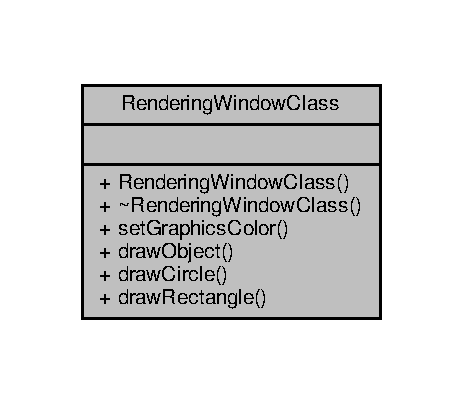
\includegraphics[width=222pt]{classRenderingWindowClass__coll__graph}
\end{center}
\end{figure}
\subsection*{Public Member Functions}
\begin{DoxyCompactItemize}
\item 
\hypertarget{classRenderingWindowClass_ad48948a08088e973aac8a57c96dee52c}{\hyperlink{classRenderingWindowClass_ad48948a08088e973aac8a57c96dee52c}{Rendering\-Window\-Class} ()}\label{classRenderingWindowClass_ad48948a08088e973aac8a57c96dee52c}

\begin{DoxyCompactList}\small\item\em Default constructor for \hyperlink{classRenderingWindowClass}{Rendering\-Window\-Class}. \end{DoxyCompactList}\item 
\hypertarget{classRenderingWindowClass_a10c28c3d432aa2e7864284301496fa85}{\hyperlink{classRenderingWindowClass_a10c28c3d432aa2e7864284301496fa85}{$\sim$\-Rendering\-Window\-Class} ()}\label{classRenderingWindowClass_a10c28c3d432aa2e7864284301496fa85}

\begin{DoxyCompactList}\small\item\em Default destructor for \hyperlink{classRenderingWindowClass}{Rendering\-Window\-Class}. \end{DoxyCompactList}\item 
double $\ast$ \hyperlink{classRenderingWindowClass_a9f6608b40171774123597e59f2a24c9c}{set\-Graphics\-Color} (\hyperlink{classPhysicalObjectClass}{Physical\-Object\-Class} $\ast$object)
\begin{DoxyCompactList}\small\item\em Determines how to render the color a \hyperlink{classPhysicalObjectClass}{Physical\-Object\-Class} object. \end{DoxyCompactList}\item 
void \hyperlink{classRenderingWindowClass_a633f976d7c799676075d3f8025c00006}{draw\-Object} (\hyperlink{classPhysicalObjectClass}{Physical\-Object\-Class} $\ast$object)
\begin{DoxyCompactList}\small\item\em Determines how to draw a \hyperlink{classPhysicalObjectClass}{Physical\-Object\-Class} object. \end{DoxyCompactList}\item 
void \hyperlink{classRenderingWindowClass_af5d9c9b8ffed253fed1a60d7720c871a}{draw\-Circle} (\hyperlink{classPhysicalObjectClass}{Physical\-Object\-Class} $\ast$object)
\begin{DoxyCompactList}\small\item\em Draws a circular object. \end{DoxyCompactList}\item 
void \hyperlink{classRenderingWindowClass_a2fa407ff2e2467edcda4f18df7531db3}{draw\-Rectangle} (\hyperlink{classPhysicalObjectClass}{Physical\-Object\-Class} $\ast$object)
\begin{DoxyCompactList}\small\item\em Draws a rectangular object. \end{DoxyCompactList}\end{DoxyCompactItemize}


\subsection{Member Function Documentation}
\hypertarget{classRenderingWindowClass_af5d9c9b8ffed253fed1a60d7720c871a}{\index{Rendering\-Window\-Class@{Rendering\-Window\-Class}!draw\-Circle@{draw\-Circle}}
\index{draw\-Circle@{draw\-Circle}!RenderingWindowClass@{Rendering\-Window\-Class}}
\subsubsection[{draw\-Circle}]{\setlength{\rightskip}{0pt plus 5cm}void Rendering\-Window\-Class\-::draw\-Circle (
\begin{DoxyParamCaption}
\item[{{\bf Physical\-Object\-Class} $\ast$}]{object}
\end{DoxyParamCaption}
)}}\label{classRenderingWindowClass_af5d9c9b8ffed253fed1a60d7720c871a}


Draws a circular object. 

This function takes in a \hyperlink{classPhysicalObjectClass}{Physical\-Object\-Class} object and draws it as a circle of radius \char`\"{}size\char`\"{} using 50 triangle fans using G\-L\-\_\-\-T\-R\-I\-A\-N\-G\-L\-E\-\_\-\-F\-A\-N. The size, color, and location are determined by the object's own attributes.


\begin{DoxyParams}{Parameters}
{\em object} & an object within the simulation\\
\hline
\end{DoxyParams}
\begin{DoxyAuthor}{Author}
Nicole Zhang 
\end{DoxyAuthor}
\hypertarget{classRenderingWindowClass_a633f976d7c799676075d3f8025c00006}{\index{Rendering\-Window\-Class@{Rendering\-Window\-Class}!draw\-Object@{draw\-Object}}
\index{draw\-Object@{draw\-Object}!RenderingWindowClass@{Rendering\-Window\-Class}}
\subsubsection[{draw\-Object}]{\setlength{\rightskip}{0pt plus 5cm}void Rendering\-Window\-Class\-::draw\-Object (
\begin{DoxyParamCaption}
\item[{{\bf Physical\-Object\-Class} $\ast$}]{object}
\end{DoxyParamCaption}
)}}\label{classRenderingWindowClass_a633f976d7c799676075d3f8025c00006}


Determines how to draw a \hyperlink{classPhysicalObjectClass}{Physical\-Object\-Class} object. 

This function takes in a \hyperlink{classPhysicalObjectClass}{Physical\-Object\-Class} object as an argument and decides based on the object's Object\-Type attribute (ball\-Type, paddle\-Type, or brick\-Type) whether to draw the object as a circle or rectangle. If an invalid Object\-Type is detected, no object is drawn.


\begin{DoxyParams}{Parameters}
{\em object} & a \hyperlink{classPhysicalObjectClass}{Physical\-Object\-Class} object within the simulation\\
\hline
\end{DoxyParams}
\begin{DoxyAuthor}{Author}
Nicole Zhang 
\end{DoxyAuthor}
\hypertarget{classRenderingWindowClass_a2fa407ff2e2467edcda4f18df7531db3}{\index{Rendering\-Window\-Class@{Rendering\-Window\-Class}!draw\-Rectangle@{draw\-Rectangle}}
\index{draw\-Rectangle@{draw\-Rectangle}!RenderingWindowClass@{Rendering\-Window\-Class}}
\subsubsection[{draw\-Rectangle}]{\setlength{\rightskip}{0pt plus 5cm}void Rendering\-Window\-Class\-::draw\-Rectangle (
\begin{DoxyParamCaption}
\item[{{\bf Physical\-Object\-Class} $\ast$}]{object}
\end{DoxyParamCaption}
)}}\label{classRenderingWindowClass_a2fa407ff2e2467edcda4f18df7531db3}


Draws a rectangular object. 

This function takes in a \hyperlink{classPhysicalObjectClass}{Physical\-Object\-Class} object and draws it as a G\-L\-\_\-\-Q\-U\-A\-D\-S. Its width, height, color, and location are all dependent on the input object's own attributes.


\begin{DoxyParams}{Parameters}
{\em object} & an object within the simulation\\
\hline
\end{DoxyParams}
\begin{DoxyAuthor}{Author}
Nicole Zhang 
\end{DoxyAuthor}
\hypertarget{classRenderingWindowClass_a9f6608b40171774123597e59f2a24c9c}{\index{Rendering\-Window\-Class@{Rendering\-Window\-Class}!set\-Graphics\-Color@{set\-Graphics\-Color}}
\index{set\-Graphics\-Color@{set\-Graphics\-Color}!RenderingWindowClass@{Rendering\-Window\-Class}}
\subsubsection[{set\-Graphics\-Color}]{\setlength{\rightskip}{0pt plus 5cm}double $\ast$ Rendering\-Window\-Class\-::set\-Graphics\-Color (
\begin{DoxyParamCaption}
\item[{{\bf Physical\-Object\-Class} $\ast$}]{object}
\end{DoxyParamCaption}
)}}\label{classRenderingWindowClass_a9f6608b40171774123597e59f2a24c9c}


Determines how to render the color a \hyperlink{classPhysicalObjectClass}{Physical\-Object\-Class} object. 

This function takes in a \hyperlink{classPhysicalObjectClass}{Physical\-Object\-Class} object as an argument and decides based on the object's color attribute which parameters to pass to G\-L\-U\-T's gl\-Color3f function, which is called in the draw\-Circle and draw\-Rectangle method.


\begin{DoxyParams}{Parameters}
{\em object} & a \hyperlink{classPhysicalObjectClass}{Physical\-Object\-Class} object within the simulation\\
\hline
\end{DoxyParams}
\begin{DoxyReturn}{Returns}
array with R\-G\-B values
\end{DoxyReturn}
\begin{DoxyAuthor}{Author}
Nicole Zhang 

Rachel Soble 
\end{DoxyAuthor}


The documentation for this class was generated from the following files\-:\begin{DoxyCompactItemize}
\item 
\hyperlink{RenderingWindowClass_8h}{Rendering\-Window\-Class.\-h}\item 
\hyperlink{RenderingWindowClass_8cpp}{Rendering\-Window\-Class.\-cpp}\end{DoxyCompactItemize}

\hypertarget{classSimulation}{\section{Simulation Class Reference}
\label{classSimulation}\index{Simulation@{Simulation}}
}


{\ttfamily \#include $<$Simulation.\-h$>$}



Inheritance diagram for Simulation\-:\nopagebreak
\begin{figure}[H]
\begin{center}
\leavevmode
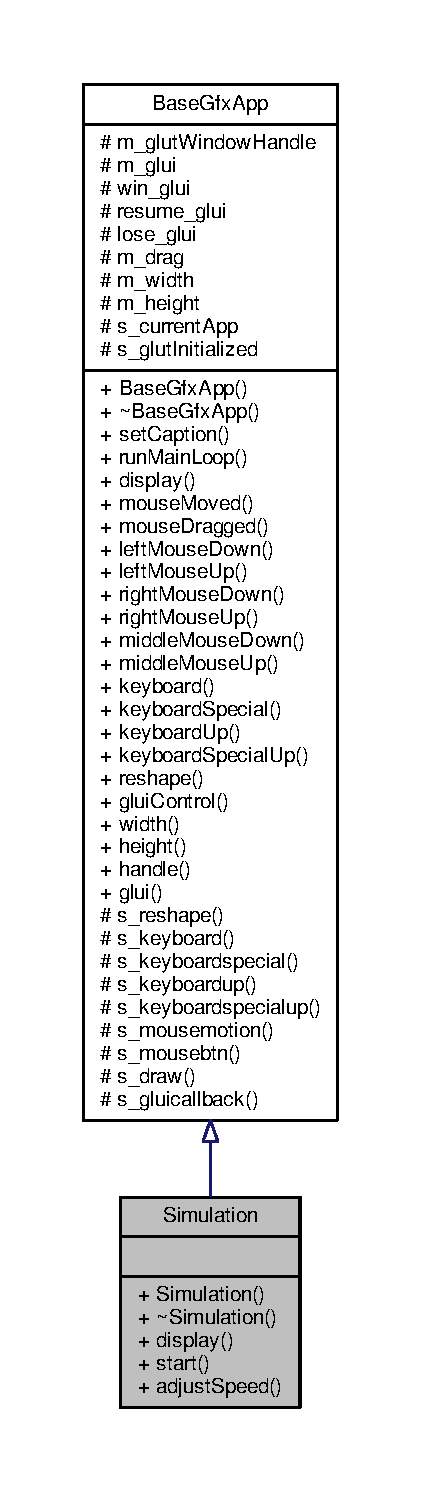
\includegraphics[height=550pt]{classSimulation__inherit__graph}
\end{center}
\end{figure}


Collaboration diagram for Simulation\-:\nopagebreak
\begin{figure}[H]
\begin{center}
\leavevmode
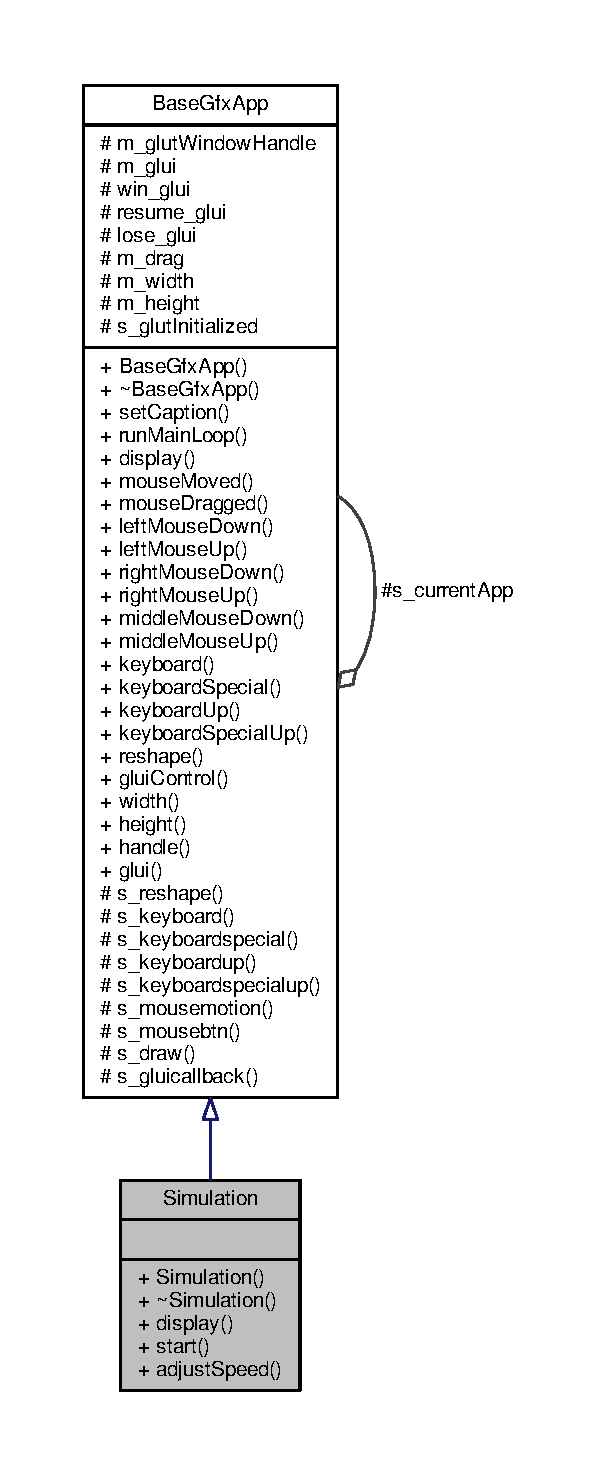
\includegraphics[height=550pt]{classSimulation__coll__graph}
\end{center}
\end{figure}
\subsection*{Public Types}
\begin{DoxyCompactItemize}
\item 
enum {\bfseries U\-I\-Control\-Type} \{ {\bfseries U\-I\-\_\-\-Q\-U\-I\-T} = 0
 \}
\end{DoxyCompactItemize}
\subsection*{Public Member Functions}
\begin{DoxyCompactItemize}
\item 
\hyperlink{classSimulation_a4c669ceaa34c7130966ce45f9de75fbe}{Simulation} (int argc, char $\ast$argv\mbox{[}$\,$\mbox{]}, int width, int height)
\begin{DoxyCompactList}\small\item\em Initializes Open\-G\-L window. \end{DoxyCompactList}\item 
\hypertarget{classSimulation_a80fad3f57dfaf195a36f7bc49bc88279}{virtual \hyperlink{classSimulation_a80fad3f57dfaf195a36f7bc49bc88279}{$\sim$\-Simulation} ()}\label{classSimulation_a80fad3f57dfaf195a36f7bc49bc88279}

\begin{DoxyCompactList}\small\item\em Default destructor. \end{DoxyCompactList}\item 
void \hyperlink{classSimulation_a449dcb7d97dfba99efe770de2f399c31}{display} ()
\begin{DoxyCompactList}\small\item\em Displays the simulation. \end{DoxyCompactList}\end{DoxyCompactItemize}
\subsection*{Static Public Member Functions}
\begin{DoxyCompactItemize}
\item 
static void \hyperlink{classSimulation_acf598e815ded8ca12cad5db975ac8849}{start} ()
\begin{DoxyCompactList}\small\item\em Starts simulation. \end{DoxyCompactList}\item 
static void \hyperlink{classSimulation_a685b3dae9c7d04df7783e2f029e3dec0}{adjust\-Speed} ()
\begin{DoxyCompactList}\small\item\em Lets user increase speed of all robots. \end{DoxyCompactList}\end{DoxyCompactItemize}
\subsection*{Additional Inherited Members}


\subsection{Detailed Description}
The \hyperlink{classSimulation}{Simulation} class. This sets up the G\-U\-I and the drawing environment. 

\subsection{Constructor \& Destructor Documentation}
\hypertarget{classSimulation_a4c669ceaa34c7130966ce45f9de75fbe}{\index{Simulation@{Simulation}!Simulation@{Simulation}}
\index{Simulation@{Simulation}!Simulation@{Simulation}}
\subsubsection[{Simulation}]{\setlength{\rightskip}{0pt plus 5cm}Simulation\-::\-Simulation (
\begin{DoxyParamCaption}
\item[{int}]{argc, }
\item[{char $\ast$}]{argv\mbox{[}$\,$\mbox{]}, }
\item[{int}]{width, }
\item[{int}]{height}
\end{DoxyParamCaption}
)}}\label{classSimulation_a4c669ceaa34c7130966ce45f9de75fbe}


Initializes Open\-G\-L window. 

Creates Open\-G\-L window and U\-I panel with Start and Quit buttons, instructions, and a speed adjuster.

\begin{DoxyAuthor}{Author}
Nicole Zhang 
\end{DoxyAuthor}


\subsection{Member Function Documentation}
\hypertarget{classSimulation_a685b3dae9c7d04df7783e2f029e3dec0}{\index{Simulation@{Simulation}!adjust\-Speed@{adjust\-Speed}}
\index{adjust\-Speed@{adjust\-Speed}!Simulation@{Simulation}}
\subsubsection[{adjust\-Speed}]{\setlength{\rightskip}{0pt plus 5cm}void Simulation\-::adjust\-Speed (
\begin{DoxyParamCaption}
{}
\end{DoxyParamCaption}
)\hspace{0.3cm}{\ttfamily [static]}}}\label{classSimulation_a685b3dae9c7d04df7783e2f029e3dec0}


Lets user increase speed of all robots. 

This function increases the speed of all robots by increasing a global flag. Once changed, this flag is added into the calculations performed in translate robot

\begin{DoxyAuthor}{Author}
Nicholas Inman 
\end{DoxyAuthor}
\hypertarget{classSimulation_a449dcb7d97dfba99efe770de2f399c31}{\index{Simulation@{Simulation}!display@{display}}
\index{display@{display}!Simulation@{Simulation}}
\subsubsection[{display}]{\setlength{\rightskip}{0pt plus 5cm}void Simulation\-::display (
\begin{DoxyParamCaption}
{}
\end{DoxyParamCaption}
)\hspace{0.3cm}{\ttfamily [virtual]}}}\label{classSimulation_a449dcb7d97dfba99efe770de2f399c31}


Displays the simulation. 

This function first determines which G\-L\-U\-I windows need to be displayed based on varying flags. Then, it calculates the passed time in the simulation and displays the environment and objects accordingly by calling the \hyperlink{classEnvironmentClass}{Environment\-Class} display function.

\begin{DoxyAuthor}{Author}
Nicole Zhang 
\end{DoxyAuthor}


Reimplemented from \hyperlink{classBaseGfxApp}{Base\-Gfx\-App}.

\hypertarget{classSimulation_acf598e815ded8ca12cad5db975ac8849}{\index{Simulation@{Simulation}!start@{start}}
\index{start@{start}!Simulation@{Simulation}}
\subsubsection[{start}]{\setlength{\rightskip}{0pt plus 5cm}void Simulation\-::start (
\begin{DoxyParamCaption}
{}
\end{DoxyParamCaption}
)\hspace{0.3cm}{\ttfamily [static]}}}\label{classSimulation_acf598e815ded8ca12cad5db975ac8849}


Starts simulation. 

Starts simulation by toggling flag. This allows the environment to run the update function and move the objects.

\begin{DoxyAuthor}{Author}
Nicholas Inman 

Nicole Zhang 
\end{DoxyAuthor}


The documentation for this class was generated from the following files\-:\begin{DoxyCompactItemize}
\item 
\hyperlink{Simulation_8h}{Simulation.\-h}\item 
\hyperlink{Simulation_8cpp}{Simulation.\-cpp}\end{DoxyCompactItemize}

\chapter{File Documentation}
\hypertarget{BaseGfxApp_8h}{\section{Base\-Gfx\-App.\-h File Reference}
\label{BaseGfxApp_8h}\index{Base\-Gfx\-App.\-h@{Base\-Gfx\-App.\-h}}
}


The basic application class for C\-Sci-\/3081 project. Uses G\-L\-U\-T and G\-L\-U\-I and wraps them in a nice C++ interface.  


{\ttfamily \#include $<$string$>$}\\*
{\ttfamily \#include $<$iostream$>$}\\*
{\ttfamily \#include $<$assert.\-h$>$}\\*
{\ttfamily \#include $<$G\-L/glui.\-h$>$}\\*
Include dependency graph for Base\-Gfx\-App.\-h\-:\nopagebreak
\begin{figure}[H]
\begin{center}
\leavevmode
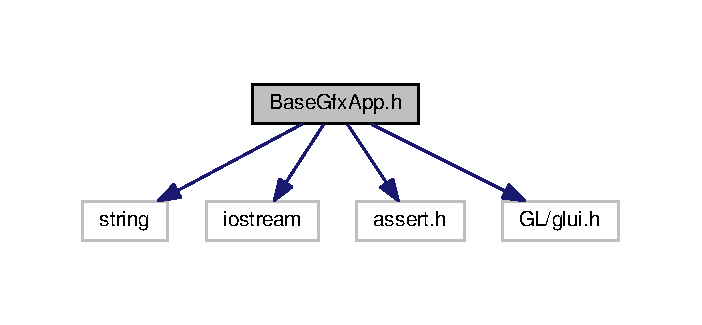
\includegraphics[width=337pt]{BaseGfxApp_8h__incl}
\end{center}
\end{figure}
This graph shows which files directly or indirectly include this file\-:\nopagebreak
\begin{figure}[H]
\begin{center}
\leavevmode
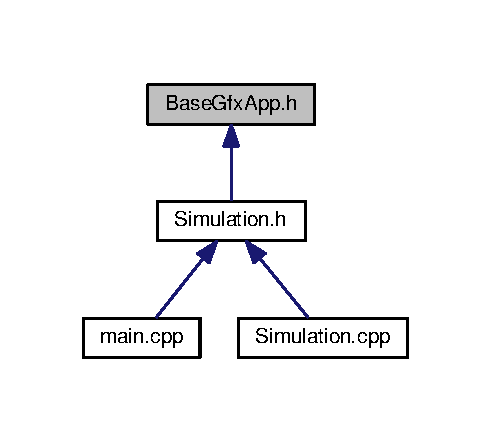
\includegraphics[width=235pt]{BaseGfxApp_8h__dep__incl}
\end{center}
\end{figure}
\subsection*{Classes}
\begin{DoxyCompactItemize}
\item 
class \hyperlink{classBaseGfxApp}{Base\-Gfx\-App}
\end{DoxyCompactItemize}
\subsection*{Variables}
\begin{DoxyCompactItemize}
\item 
\hypertarget{BaseGfxApp_8h_adf916204820072417ed73a32de1cefcf}{int {\bfseries flag}}\label{BaseGfxApp_8h_adf916204820072417ed73a32de1cefcf}

\end{DoxyCompactItemize}


\subsection{Detailed Description}
The basic application class for C\-Sci-\/3081 project. Uses G\-L\-U\-T and G\-L\-U\-I and wraps them in a nice C++ interface. \begin{DoxyAuthor}{Author}
C\-Sci3081 Guru 
\end{DoxyAuthor}

\hypertarget{EnvironmentClass_8cpp}{\section{Environment\-Class.\-cpp File Reference}
\label{EnvironmentClass_8cpp}\index{Environment\-Class.\-cpp@{Environment\-Class.\-cpp}}
}


Manages and controls object movement and behavior.  


{\ttfamily \#include \char`\"{}Environment\-Class.\-h\char`\"{}}\\*
Include dependency graph for Environment\-Class.\-cpp\-:\nopagebreak
\begin{figure}[H]
\begin{center}
\leavevmode
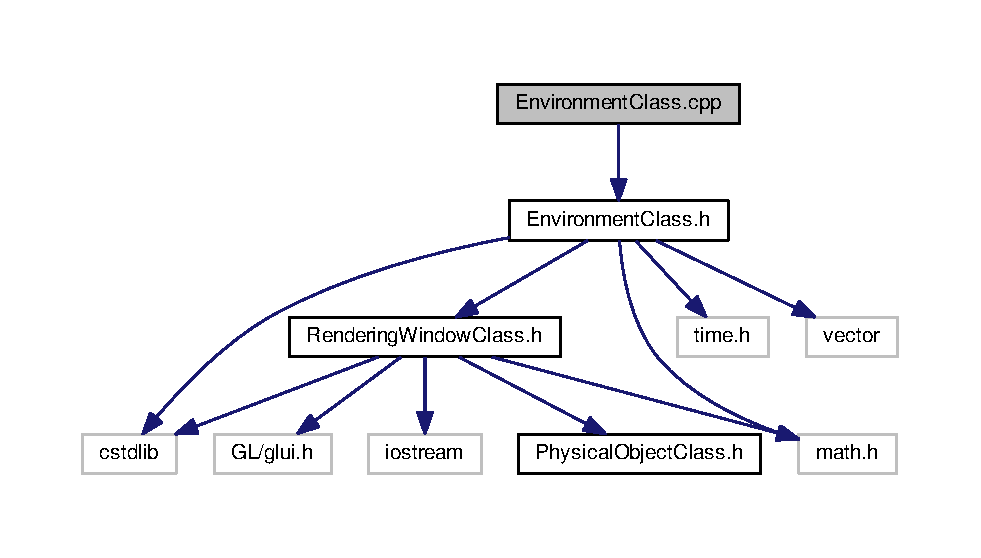
\includegraphics[width=350pt]{EnvironmentClass_8cpp__incl}
\end{center}
\end{figure}
\subsection*{Variables}
\begin{DoxyCompactItemize}
\item 
\hypertarget{EnvironmentClass_8cpp_a7fee7b546595edcbee920757b6309386}{int {\bfseries win} = 0}\label{EnvironmentClass_8cpp_a7fee7b546595edcbee920757b6309386}

\item 
\hypertarget{EnvironmentClass_8cpp_aca88a52dae5a5f74cfaa56c90eb86abb}{int {\bfseries lose} = 0}\label{EnvironmentClass_8cpp_aca88a52dae5a5f74cfaa56c90eb86abb}

\item 
\hypertarget{EnvironmentClass_8cpp_acbd8fcac2ddb57fb013fc17fb583015e}{int {\bfseries lost\-Life} = 0}\label{EnvironmentClass_8cpp_acbd8fcac2ddb57fb013fc17fb583015e}

\end{DoxyCompactItemize}


\subsection{Detailed Description}
Manages and controls object movement and behavior. 
\hypertarget{EnvironmentClass_8h}{\section{Environment\-Class.\-h File Reference}
\label{EnvironmentClass_8h}\index{Environment\-Class.\-h@{Environment\-Class.\-h}}
}


The class that controls the environment that the objects move in.  


{\ttfamily \#include \char`\"{}Rendering\-Window\-Class.\-h\char`\"{}}\\*
{\ttfamily \#include $<$time.\-h$>$}\\*
{\ttfamily \#include $<$math.\-h$>$}\\*
{\ttfamily \#include $<$vector$>$}\\*
{\ttfamily \#include $<$cstdlib$>$}\\*
Include dependency graph for Environment\-Class.\-h\-:\nopagebreak
\begin{figure}[H]
\begin{center}
\leavevmode
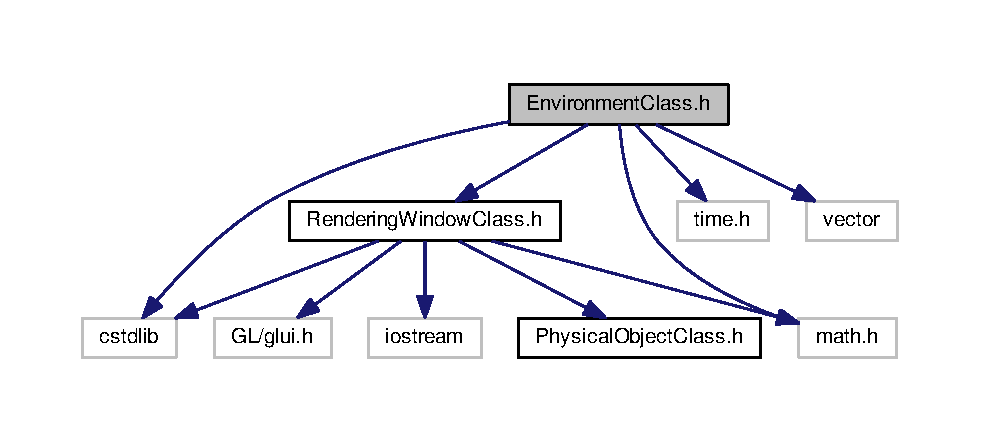
\includegraphics[width=350pt]{EnvironmentClass_8h__incl}
\end{center}
\end{figure}
This graph shows which files directly or indirectly include this file\-:\nopagebreak
\begin{figure}[H]
\begin{center}
\leavevmode
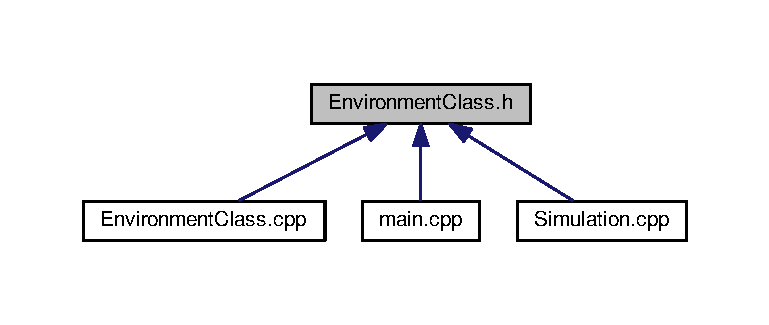
\includegraphics[width=350pt]{EnvironmentClass_8h__dep__incl}
\end{center}
\end{figure}
\subsection*{Classes}
\begin{DoxyCompactItemize}
\item 
class \hyperlink{classEnvironmentClass}{Environment\-Class}
\end{DoxyCompactItemize}
\subsection*{Enumerations}
\begin{DoxyCompactItemize}
\item 
enum \hyperlink{EnvironmentClass_8h_aa884075f403706dceea29a61771a0d44}{Collision\-Type} \{ \\*
{\bfseries left\-Collision}, 
{\bfseries right\-Collision}, 
{\bfseries top\-Collision}, 
{\bfseries bottom\-Collision}, 
\\*
{\bfseries no\-Collision}
 \}
\begin{DoxyCompactList}\small\item\em Relative collision locations on a brick. \end{DoxyCompactList}\end{DoxyCompactItemize}
\subsection*{Variables}
\begin{DoxyCompactItemize}
\item 
\hypertarget{EnvironmentClass_8h_adf916204820072417ed73a32de1cefcf}{int {\bfseries flag}}\label{EnvironmentClass_8h_adf916204820072417ed73a32de1cefcf}

\item 
\hypertarget{EnvironmentClass_8h_a507238b0429f1503b4fefcc93c17aa0c}{float {\bfseries user\-Speed}}\label{EnvironmentClass_8h_a507238b0429f1503b4fefcc93c17aa0c}

\item 
\hypertarget{EnvironmentClass_8h_ac1d68ef9a5dd304c5015e07af7f2bb19}{int {\bfseries lives}}\label{EnvironmentClass_8h_ac1d68ef9a5dd304c5015e07af7f2bb19}

\item 
\hypertarget{EnvironmentClass_8h_a68acc917c8e6e7257bac4c39d7dd1083}{int {\bfseries paddle\-Movement}}\label{EnvironmentClass_8h_a68acc917c8e6e7257bac4c39d7dd1083}

\item 
\hypertarget{EnvironmentClass_8h_aa61000540636bfdc4c9f27045ab84ce9}{int {\bfseries window\-Width}}\label{EnvironmentClass_8h_aa61000540636bfdc4c9f27045ab84ce9}

\item 
\hypertarget{EnvironmentClass_8h_af140802328ffe8a45749114b1c5a2056}{int {\bfseries window\-Height}}\label{EnvironmentClass_8h_af140802328ffe8a45749114b1c5a2056}

\end{DoxyCompactItemize}


\subsection{Detailed Description}
The class that controls the environment that the objects move in. Environment Class header 
\hypertarget{main_8cpp}{\section{main.\-cpp File Reference}
\label{main_8cpp}\index{main.\-cpp@{main.\-cpp}}
}


driver file for robot class  


{\ttfamily \#include \char`\"{}Simulation.\-h\char`\"{}}\\*
{\ttfamily \#include \char`\"{}Environment\-Class.\-h\char`\"{}}\\*
Include dependency graph for main.\-cpp\-:\nopagebreak
\begin{figure}[H]
\begin{center}
\leavevmode
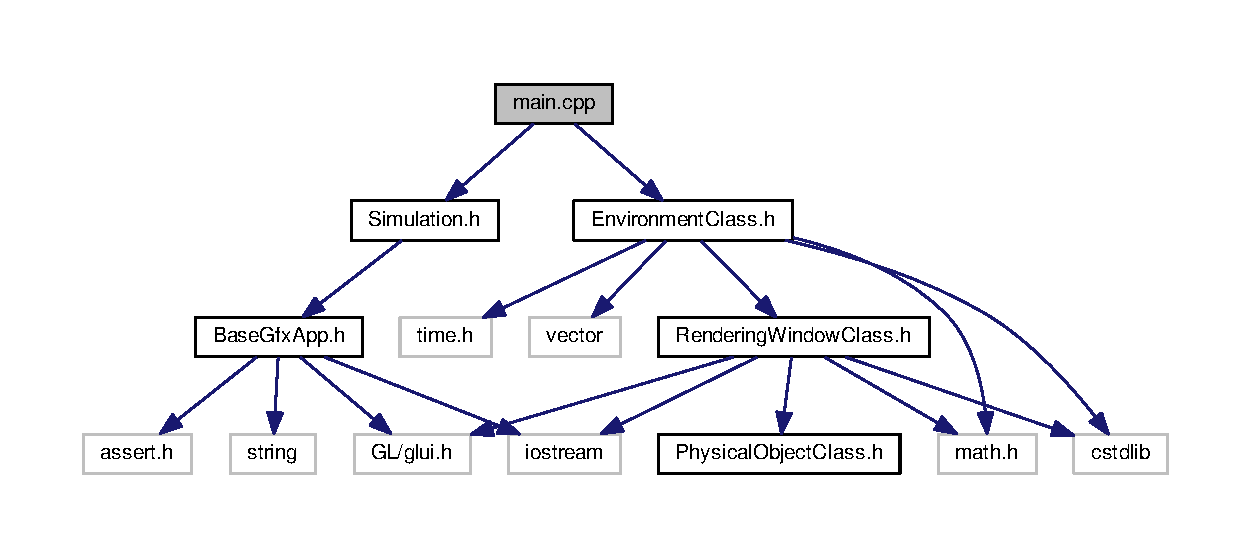
\includegraphics[width=350pt]{main_8cpp__incl}
\end{center}
\end{figure}
\subsection*{Functions}
\begin{DoxyCompactItemize}
\item 
\hypertarget{main_8cpp_a0ddf1224851353fc92bfbff6f499fa97}{int {\bfseries main} (int argc, char $\ast$argv\mbox{[}$\,$\mbox{]})}\label{main_8cpp_a0ddf1224851353fc92bfbff6f499fa97}

\end{DoxyCompactItemize}
\subsection*{Variables}
\begin{DoxyCompactItemize}
\item 
\hypertarget{main_8cpp_aa61000540636bfdc4c9f27045ab84ce9}{int {\bfseries window\-Width} = 800}\label{main_8cpp_aa61000540636bfdc4c9f27045ab84ce9}

\item 
\hypertarget{main_8cpp_af140802328ffe8a45749114b1c5a2056}{int {\bfseries window\-Height} = 600}\label{main_8cpp_af140802328ffe8a45749114b1c5a2056}

\item 
\hypertarget{main_8cpp_a4565ba47a8833e389b48398eae7d5e42}{int {\bfseries bricks\-Per\-Row} = 16}\label{main_8cpp_a4565ba47a8833e389b48398eae7d5e42}

\item 
\hypertarget{main_8cpp_a2f6afae4c05dd6436a42fffb76357b31}{int {\bfseries brick\-Width} = 800 / bricks\-Per\-Row}\label{main_8cpp_a2f6afae4c05dd6436a42fffb76357b31}

\item 
\hypertarget{main_8cpp_acf73454e8295a8e255208ccd7d4a9f5e}{int {\bfseries brick\-Height} = 15}\label{main_8cpp_acf73454e8295a8e255208ccd7d4a9f5e}

\item 
\hypertarget{main_8cpp_ac71454c9f281c2194ba95a90097e4751}{int {\bfseries num\-Bricks} = bricks\-Per\-Row $\ast$ 6}\label{main_8cpp_ac71454c9f281c2194ba95a90097e4751}

\item 
\hypertarget{main_8cpp_ac1d68ef9a5dd304c5015e07af7f2bb19}{int {\bfseries lives} = 3}\label{main_8cpp_ac1d68ef9a5dd304c5015e07af7f2bb19}

\item 
\hypertarget{main_8cpp_adf916204820072417ed73a32de1cefcf}{int {\bfseries flag} = 1}\label{main_8cpp_adf916204820072417ed73a32de1cefcf}

\item 
\hypertarget{main_8cpp_a096533d53bd51a3ea732f287f8dbf003}{double {\bfseries past\-Time} = 0}\label{main_8cpp_a096533d53bd51a3ea732f287f8dbf003}

\item 
\hypertarget{main_8cpp_a507238b0429f1503b4fefcc93c17aa0c}{float {\bfseries user\-Speed} = 0}\label{main_8cpp_a507238b0429f1503b4fefcc93c17aa0c}

\item 
\hypertarget{main_8cpp_a76b4da66db3ceb6375487da9edcf122b}{\hyperlink{classEnvironmentClass}{Environment\-Class} {\bfseries environment}}\label{main_8cpp_a76b4da66db3ceb6375487da9edcf122b}

\end{DoxyCompactItemize}


\subsection{Detailed Description}
driver file for robot class Creates objects and runs simulation loop

\begin{DoxyAuthor}{Author}
Nicole Zhang 
\end{DoxyAuthor}

\hypertarget{PhysicalObjectClass_8cpp}{\section{Physical\-Object\-Class.\-cpp File Reference}
\label{PhysicalObjectClass_8cpp}\index{Physical\-Object\-Class.\-cpp@{Physical\-Object\-Class.\-cpp}}
}


The class that creates all physical objects.  


{\ttfamily \#include \char`\"{}Physical\-Object\-Class.\-h\char`\"{}}\\*
{\ttfamily \#include $<$cstdlib$>$}\\*
{\ttfamily \#include $<$iostream$>$}\\*
Include dependency graph for Physical\-Object\-Class.\-cpp\-:\nopagebreak
\begin{figure}[H]
\begin{center}
\leavevmode
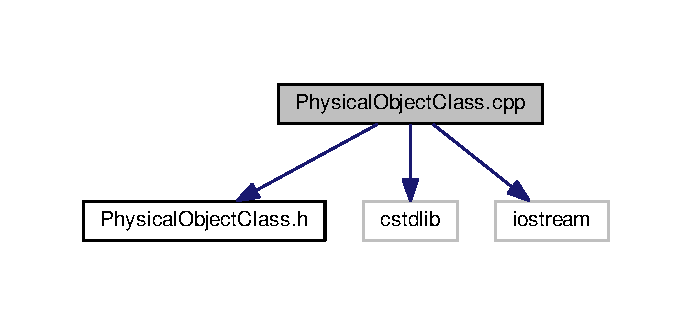
\includegraphics[width=332pt]{PhysicalObjectClass_8cpp__incl}
\end{center}
\end{figure}


\subsection{Detailed Description}
The class that creates all physical objects. \hyperlink{PhysicalObjectClass_8cpp}{Physical\-Object\-Class.\-cpp} 
\hypertarget{PhysicalObjectClass_8h}{\section{Physical\-Object\-Class.\-h File Reference}
\label{PhysicalObjectClass_8h}\index{Physical\-Object\-Class.\-h@{Physical\-Object\-Class.\-h}}
}


The class that creates all physical objects.  


This graph shows which files directly or indirectly include this file\-:\nopagebreak
\begin{figure}[H]
\begin{center}
\leavevmode
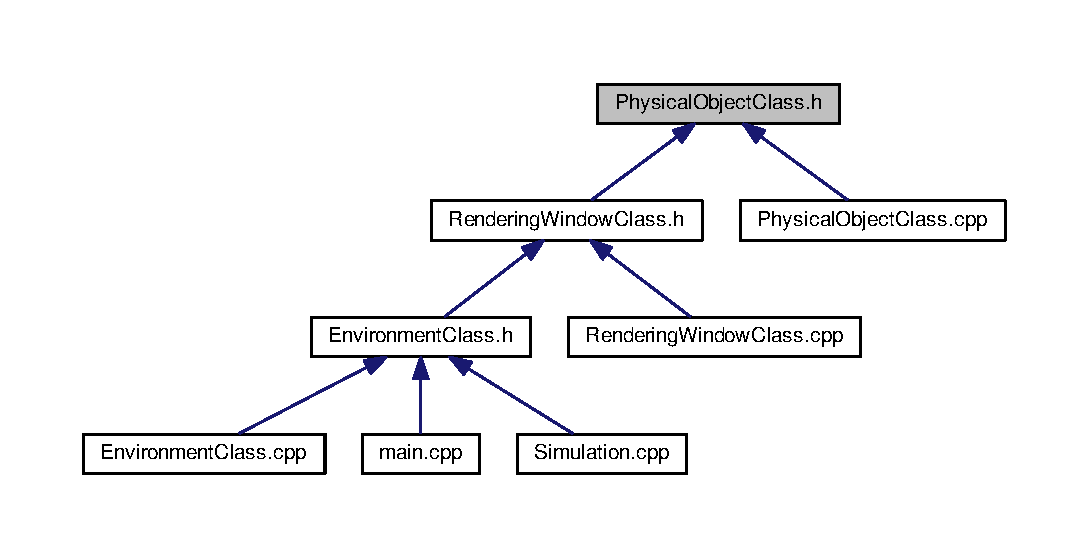
\includegraphics[width=350pt]{PhysicalObjectClass_8h__dep__incl}
\end{center}
\end{figure}
\subsection*{Classes}
\begin{DoxyCompactItemize}
\item 
class \hyperlink{classPhysicalObjectClass}{Physical\-Object\-Class}
\end{DoxyCompactItemize}
\subsection*{Enumerations}
\begin{DoxyCompactItemize}
\item 
enum \hyperlink{PhysicalObjectClass_8h_a842c5e2e69277690b064bf363c017980}{Object\-Type} \{ {\bfseries ball\-Type}, 
{\bfseries paddle\-Type}, 
{\bfseries brick\-Type}
 \}
\begin{DoxyCompactList}\small\item\em Different object types of Physical\-Ojbects. \end{DoxyCompactList}\end{DoxyCompactItemize}
\subsection*{Variables}
\begin{DoxyCompactItemize}
\item 
\hypertarget{PhysicalObjectClass_8h_a76b4da66db3ceb6375487da9edcf122b}{\hyperlink{classEnvironmentClass}{Environment\-Class} {\bfseries environment}}\label{PhysicalObjectClass_8h_a76b4da66db3ceb6375487da9edcf122b}

\item 
\hypertarget{PhysicalObjectClass_8h_a2f6afae4c05dd6436a42fffb76357b31}{int {\bfseries brick\-Width}}\label{PhysicalObjectClass_8h_a2f6afae4c05dd6436a42fffb76357b31}

\item 
\hypertarget{PhysicalObjectClass_8h_acf73454e8295a8e255208ccd7d4a9f5e}{int {\bfseries brick\-Height}}\label{PhysicalObjectClass_8h_acf73454e8295a8e255208ccd7d4a9f5e}

\end{DoxyCompactItemize}


\subsection{Detailed Description}
The class that creates all physical objects. \hyperlink{classPhysicalObjectClass}{Physical\-Object\-Class} header 
\hypertarget{RenderingWindowClass_8cpp}{\section{Rendering\-Window\-Class.\-cpp File Reference}
\label{RenderingWindowClass_8cpp}\index{Rendering\-Window\-Class.\-cpp@{Rendering\-Window\-Class.\-cpp}}
}


Interface between the graphics and \hyperlink{classEnvironmentClass}{Environment\-Class}.  


{\ttfamily \#include \char`\"{}Rendering\-Window\-Class.\-h\char`\"{}}\\*
Include dependency graph for Rendering\-Window\-Class.\-cpp\-:\nopagebreak
\begin{figure}[H]
\begin{center}
\leavevmode
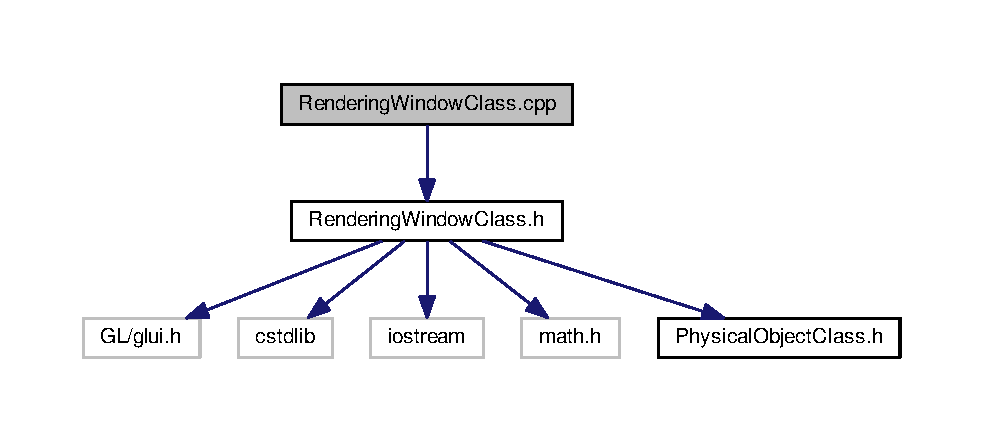
\includegraphics[width=350pt]{RenderingWindowClass_8cpp__incl}
\end{center}
\end{figure}
\subsection*{Macros}
\begin{DoxyCompactItemize}
\item 
\hypertarget{RenderingWindowClass_8cpp_a598a3330b3c21701223ee0ca14316eca}{\#define {\bfseries P\-I}~3.\-14f}\label{RenderingWindowClass_8cpp_a598a3330b3c21701223ee0ca14316eca}

\end{DoxyCompactItemize}


\subsection{Detailed Description}
Interface between the graphics and \hyperlink{classEnvironmentClass}{Environment\-Class}. \hyperlink{RenderingWindowClass_8cpp}{Rendering\-Window\-Class.\-cpp} 
\hypertarget{RenderingWindowClass_8h}{\section{Rendering\-Window\-Class.\-h File Reference}
\label{RenderingWindowClass_8h}\index{Rendering\-Window\-Class.\-h@{Rendering\-Window\-Class.\-h}}
}


Interface between the graphics and \hyperlink{classEnvironmentClass}{Environment\-Class}.  


{\ttfamily \#include $<$G\-L/glui.\-h$>$}\\*
{\ttfamily \#include $<$cstdlib$>$}\\*
{\ttfamily \#include $<$iostream$>$}\\*
{\ttfamily \#include $<$math.\-h$>$}\\*
{\ttfamily \#include \char`\"{}Physical\-Object\-Class.\-h\char`\"{}}\\*
Include dependency graph for Rendering\-Window\-Class.\-h\-:\nopagebreak
\begin{figure}[H]
\begin{center}
\leavevmode
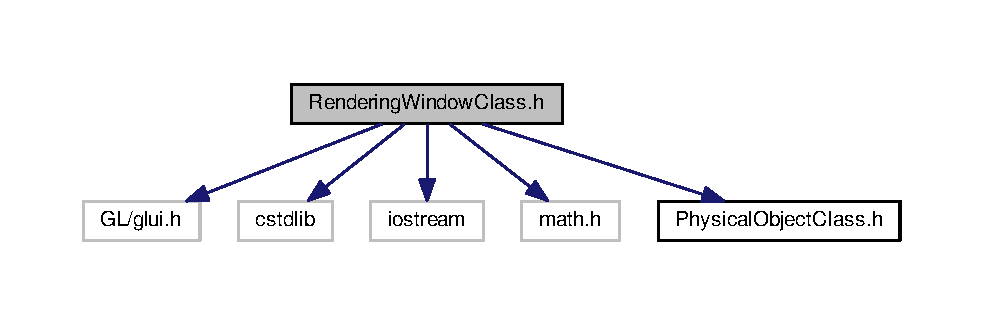
\includegraphics[width=350pt]{RenderingWindowClass_8h__incl}
\end{center}
\end{figure}
This graph shows which files directly or indirectly include this file\-:\nopagebreak
\begin{figure}[H]
\begin{center}
\leavevmode
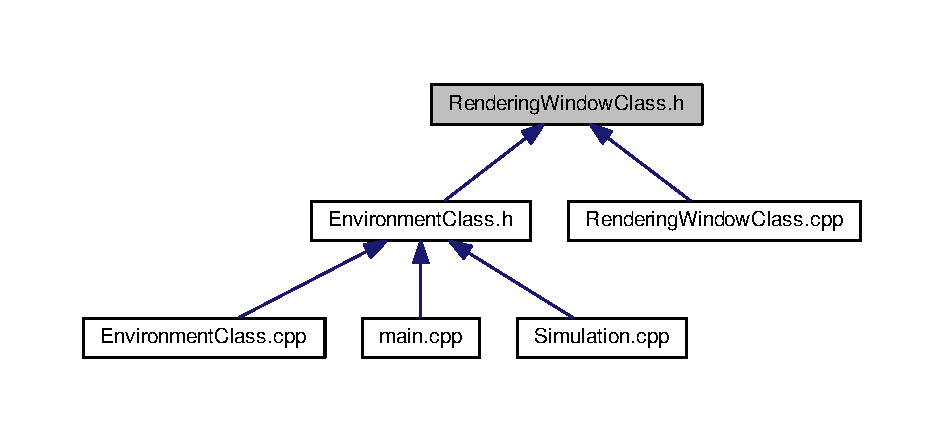
\includegraphics[width=350pt]{RenderingWindowClass_8h__dep__incl}
\end{center}
\end{figure}
\subsection*{Classes}
\begin{DoxyCompactItemize}
\item 
class \hyperlink{classRenderingWindowClass}{Rendering\-Window\-Class}
\end{DoxyCompactItemize}


\subsection{Detailed Description}
Interface between the graphics and \hyperlink{classEnvironmentClass}{Environment\-Class}. \hyperlink{classRenderingWindowClass}{Rendering\-Window\-Class} header 
\hypertarget{Simulation_8cpp}{\section{Simulation.\-cpp File Reference}
\label{Simulation_8cpp}\index{Simulation.\-cpp@{Simulation.\-cpp}}
}


Contains \hyperlink{classSimulation}{Simulation} class definitions.  


{\ttfamily \#include \char`\"{}Simulation.\-h\char`\"{}}\\*
{\ttfamily \#include \char`\"{}Environment\-Class.\-h\char`\"{}}\\*
Include dependency graph for Simulation.\-cpp\-:\nopagebreak
\begin{figure}[H]
\begin{center}
\leavevmode
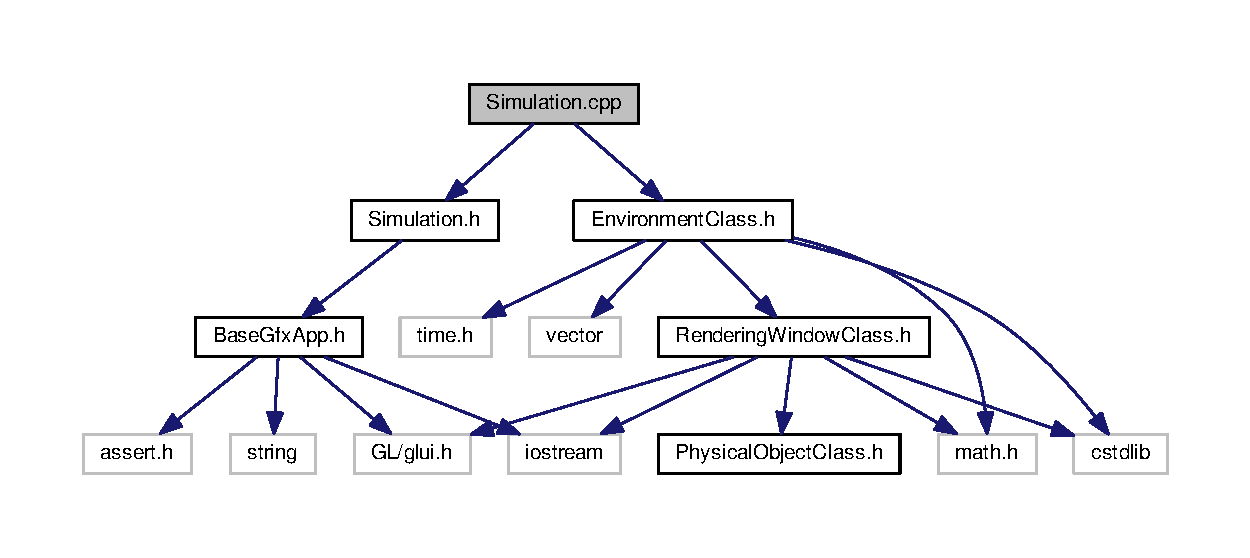
\includegraphics[width=350pt]{Simulation_8cpp__incl}
\end{center}
\end{figure}
\subsection*{Macros}
\begin{DoxyCompactItemize}
\item 
\hypertarget{Simulation_8cpp_a598a3330b3c21701223ee0ca14316eca}{\#define {\bfseries P\-I}~3.\-14}\label{Simulation_8cpp_a598a3330b3c21701223ee0ca14316eca}

\end{DoxyCompactItemize}


\subsection{Detailed Description}
Contains \hyperlink{classSimulation}{Simulation} class definitions. 
\hypertarget{Simulation_8h}{\section{Simulation.\-h File Reference}
\label{Simulation_8h}\index{Simulation.\-h@{Simulation.\-h}}
}


Main application class for the robot simulation.  


{\ttfamily \#include \char`\"{}Base\-Gfx\-App.\-h\char`\"{}}\\*
Include dependency graph for Simulation.\-h\-:\nopagebreak
\begin{figure}[H]
\begin{center}
\leavevmode
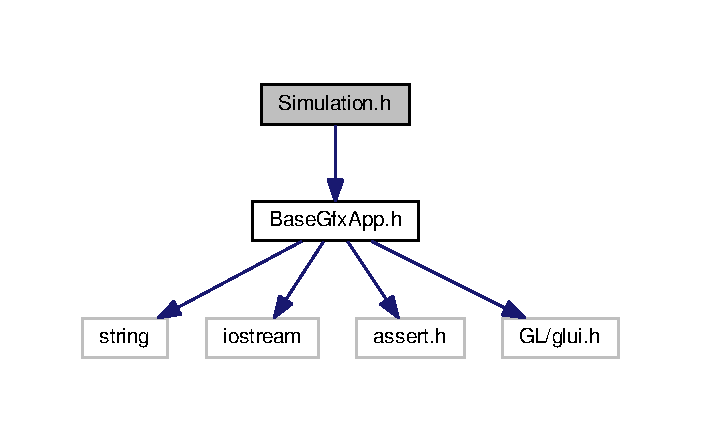
\includegraphics[width=337pt]{Simulation_8h__incl}
\end{center}
\end{figure}
This graph shows which files directly or indirectly include this file\-:\nopagebreak
\begin{figure}[H]
\begin{center}
\leavevmode
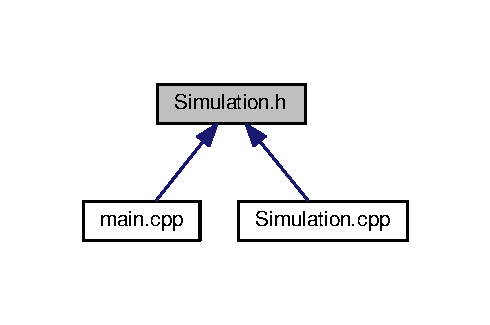
\includegraphics[width=235pt]{Simulation_8h__dep__incl}
\end{center}
\end{figure}
\subsection*{Classes}
\begin{DoxyCompactItemize}
\item 
class \hyperlink{classSimulation}{Simulation}
\end{DoxyCompactItemize}
\subsection*{Variables}
\begin{DoxyCompactItemize}
\item 
\hypertarget{Simulation_8h_a7fee7b546595edcbee920757b6309386}{int {\bfseries win}}\label{Simulation_8h_a7fee7b546595edcbee920757b6309386}

\item 
\hypertarget{Simulation_8h_aca88a52dae5a5f74cfaa56c90eb86abb}{int {\bfseries lose}}\label{Simulation_8h_aca88a52dae5a5f74cfaa56c90eb86abb}

\item 
\hypertarget{Simulation_8h_acbd8fcac2ddb57fb013fc17fb583015e}{int {\bfseries lost\-Life}}\label{Simulation_8h_acbd8fcac2ddb57fb013fc17fb583015e}

\item 
\hypertarget{Simulation_8h_ac1d68ef9a5dd304c5015e07af7f2bb19}{int {\bfseries lives}}\label{Simulation_8h_ac1d68ef9a5dd304c5015e07af7f2bb19}

\item 
\hypertarget{Simulation_8h_adf916204820072417ed73a32de1cefcf}{int {\bfseries flag}}\label{Simulation_8h_adf916204820072417ed73a32de1cefcf}

\item 
\hypertarget{Simulation_8h_a096533d53bd51a3ea732f287f8dbf003}{double {\bfseries past\-Time}}\label{Simulation_8h_a096533d53bd51a3ea732f287f8dbf003}

\item 
\hypertarget{Simulation_8h_a507238b0429f1503b4fefcc93c17aa0c}{float {\bfseries user\-Speed}}\label{Simulation_8h_a507238b0429f1503b4fefcc93c17aa0c}

\end{DoxyCompactItemize}


\subsection{Detailed Description}
Main application class for the robot simulation. \hyperlink{classSimulation}{Simulation} header 
%--- End generated contents ---

% Index
\newpage
\phantomsection
\addcontentsline{toc}{chapter}{Index}
\printindex

\end{document}
